\section{Experiments \& Results}\label{sec:methodology}
This section outlines the experimental design used to identify the top-$n$ models to be used for our stacking ensemble.
We begin with a description of the prerequisite data preparation necessary for all experiments, followed by an overview of the hardware and software used.
Next, we outline the design of our initial experiment, which provides a preliminary assessment of the models selected in Section~\ref{sec:model_selection}.
The results of this initial experiment are then presented and discussed.
We then describe the design of our main experiment.
This experiment leverages our hyperparameter tuning framework to identify the top-$n$ models. 
The results are then presented and discussed the results of this experiment.
Finally, we use the identified models to construct a stacking ensemble, which is then evaluated and compared to the individual models.

\subsection{Data Preparation}\label{sec:data-preparation}
The first step in our methodology is to prepare the datasets for model training and evaluation.
As mentioned in Section~\ref{sec:data-overview}, the data used in this study was obtained from \gls{nasa}'s \gls{pds} and consists of \gls{ccs} data and major oxide compositions for various samples.

The initial five shots from each sample are excluded because they are usually contaminated by dust covering the sample, which is cleared away by the shock waves produced by the laser \cite{cleggRecalibrationMarsScience2017}.
The remaining 45 shots from each location are then averaged, yielding a single spectrum $s$ per location $l$ in the \texttt{Averaged Intensity Tensor} (Tensor \ref{matrix:averaged_intensity}), resulting in a total of five spectra for each sample.

At this stage, the data still contains noise at the edges of the spectrometers.
These edges correspond to the boundaries of the three spectrometers, which collectively cover the \gls{uv}, \gls{vio}, and \gls{vnir} light spectra.
The noisy edge ranges are as follows: 240.811-246.635 nm, 338.457-340.797 nm, 382.138-387.859 nm, 473.184-492.427 nm, and 849-905.574 nm.
In addition to being noisy regions, these regions do not contain any useful information related to each of the major oxides.
Consequently, these regions are masked by zeroing out the values, rather than removing them, as they represent meaningful variation in the data~\cite{cleggRecalibrationMarsScience2017}.

Additionally, as a result of the aforementioned preprocessing applied to the raw \gls{libs} data, negative values are present in the \gls{ccs} data.
These negative values are not physically meaningful, since you cannot have negative light intensity \cite{p9_paper}.
Similar to the noisy edges, these negative values are also masked by zeroing out the values.

We transpose the data so that each row represents a location and each column represents a wavelength feature.
Each location is now represented as a vector of wavelengths, with the corresponding average intensity values for each wavelength.
These vectors are then concatenated to form a tensor, giving us the full \texttt{Averaged Intensity Tensor}.

For each sample, we have a corresponding set of major oxide compositions in weight percentage (wt\%).
These compositions are used as the target labels for the machine learning models.
An excerpt of this data is shown in Table \ref{tab:composition_data_example}.
While the \textit{Target}, \textit{Spectrum Name}, and \textit{Sample Names} are part of the dataset, our analysis focuses primarily on the \textit{Sample Names}.
The concentrations of the eight oxides \ce{SiO2}, \ce{TiO2}, \ce{Al2O3}, \ce{FeO_T}, \ce{MnO}, \ce{MgO}, \ce{CaO}, \ce{Na2O}, and \ce{K2O} represent the expected values for these oxides in the sample, serving as our ground truth. The \textit{MOC total} is not utilized in this study.

\begin{table*}
\centering
\caption{Excerpt from the composition dataset (from \citet{p9_paper}).}
\begin{tabular}{lllllllllllll}
\toprule
     Target & Spectrum Name & Sample Name & \ce{SiO2} & \ce{TiO2} & \ce{Al2O3} & \ce{FeO_T} & \ce{MnO} & \ce{MgO} & \ce{CaO} & \ce{Na2O} & \ce{K2O} & \ce{MOC total} \\
\midrule
AGV2 & AGV2 & AGV2 & 59.3 & 1.05 & 16.91 & 6.02 & 0.099 & 1.79 & 5.2 & 4.19 & 2.88 & 97.44 \\
BCR-2 & BCR2 & BCR2 & 54.1 & 2.26 & 13.5 & 12.42 & 0.2 & 3.59 & 7.12 & 3.16 & 1.79 & 98.14 \\
$\vdots$ & $\vdots$ & $\vdots$ & $\vdots$ & $\vdots$ & $\vdots$ & $\vdots$ & $\vdots$ & $\vdots$ & $\vdots$ & $\vdots$ & $\vdots$ & $\vdots$ \\
TB & --- & --- & 60.23 & 0.93 & 20.64 & 11.6387 & 0.052 & 1.93 & 0.000031 & 1.32 & 3.87 & 100.610731 \\
    TB2 & --- & --- & 60.4 & 0.93 & 20.5 & 11.6536 & 0.047 & 1.86 & 0.2 & 1.29 & 3.86 & 100.7406 \\
\bottomrule
\end{tabular}
\label{tab:composition_data_example}
\end{table*}

The major oxide weight percentages are appended to the matrix of spectral data, forming the final dataset.
This dataset is shown in Table~\ref{tab:final_dataset_example}.
The \textit{Target} column corresponds to the sample name, while the \textit{ID} column contains the unique identifier for each location.

\begin{table*}
\centering
\caption{Excerpt from the final dataset (values have been rounded to two decimal places for brevity).}
\footnotesize
\begin{tabular}{llllllllllllllllllllll}
\toprule
    240.81   & $\cdots$     & 425.82    & 425.87   & $\cdots$ & 905.57  & \ce{SiO2} & \ce{TiO2} & \ce{Al2O3} & \ce{FeO_T} & \ce{MgO} & \ce{CaO} & \ce{Na2O} & \ce{K2O} & Target     & ID \\
\midrule
	0        & $\cdots$     & 1.53e+10 & 1.62e+10 & $\cdots$ & 0        & 56.13     & 0.69 & 17.69 & 5.86 & 3.85 & 7.07 & 3.32 & 1.44 & jsc1421     & jsc1421\_2013\_09\_12\_211002\_ccs \\
	0        & $\cdots$     & 1.28e+10 & 1.30e+10 & $\cdots$ & 0        & 56.13     & 0.69 & 17.69 & 5.86 & 3.85 & 7.07 & 3.32 & 1.44 & jsc1421     & jsc1421\_2013\_09\_12\_211143\_ccs \\
    0        & $\cdots$     & 1.87e+10 & 1.83e+10 & $\cdots$ & 0        & 56.13     & 0.69 & 17.69 & 5.86 & 3.85 & 7.07 & 3.32 & 1.44 & jsc1421     & jsc1421\_2013\_09\_12\_210628\_ccs \\
    0        & $\cdots$     & 1.77e+10 & 1.78e+10 & $\cdots$ & 0        & 56.13     & 0.69 & 17.69 & 5.86 & 3.85 & 7.07 & 3.32 & 1.44 & jsc1421     & jsc1421\_2013\_09\_12\_210415\_ccs \\
    0        & $\cdots$     & 1.75e+10 & 1.79e+10 & $\cdots$ & 0        & 56.13     & 0.69 & 17.69 & 5.86 & 3.85 & 7.07 & 3.32 & 1.44 & jsc1421     & jsc1421\_2013\_09\_12\_210811\_ccs \\
    0        & $\cdots$     & 5.52e+10 & 3.74e+10 & $\cdots$ & 0        & 57.60     & 0.78 & 26.60 & 2.73 & 0.70 & 0.01 & 0.38 & 7.10 & pg7         & pg7\_2013\_11\_07\_161903\_ccs \\
    0        & $\cdots$     & 5.09e+10 & 3.41e+10 & $\cdots$ & 0        & 57.60     & 0.78 & 26.60 & 2.73 & 0.70 & 0.01 & 0.38 & 7.10 & pg7         & pg7\_2013\_11\_07\_162038\_ccs \\
    0        & $\cdots$     & 5.99e+10 & 3.97e+10 & $\cdots$ & 0        & 57.60     & 0.78 & 26.60 & 2.73 & 0.70 & 0.01 & 0.38 & 7.10 & pg7         & pg7\_2013\_11\_07\_161422\_ccs \\
    0        & $\cdots$     & 5.22e+10 & 3.47e+10 & $\cdots$ & 0        & 57.60     & 0.78 & 26.60 & 2.73 & 0.70 & 0.01 & 0.38 & 7.10 & pg7         & pg7\_2013\_11\_07\_161735\_ccs \\
    0        & $\cdots$     & 5.29e+10 & 3.62e+10 & $\cdots$ & 0        & 57.60     & 0.78 & 26.60 & 2.73 & 0.70 & 0.01 & 0.38 & 7.10 & pg7         & pg7\_2013\_11\_07\_161552\_ccs \\
	$\vdots$ & $\cdots$ & $\vdots$ & $\vdots$ & $\cdots$ & $\vdots$ & $\vdots$ & $\vdots$ & $\vdots$ & $\vdots$ & $\vdots$ & $\vdots$ & $\vdots$ & $\vdots$ & $\vdots$ & $\vdots$ \\
\midrule
\end{tabular}
\label{tab:final_dataset_example}
\end{table*}
\subsection{Experimental Setup}
Experiments were conducted on a machine equipped with an Intel Xeon Gold 6242 CPU, featuring 16 cores and 32 threads.
The CPU has a base clock speed of 2.80 GHz and a maximum turbo frequency of 3.90 GHz.
The system has 64 GB of RAM and runs on Ubuntu 22.04.2 LTS.
Models were implemented using Python 3.10.11.
The primary libraries used were Scikit-learn 1.4.2, XGBoost 2.0.3, Torch 2.2.2, NumPy 1.26.4, Pandas 2.2.1, Keras 3.2.1 and Optuna 3.6.1.
Additionally, all experiments were run using the hyperparameter optimization tool described in Section~\ref{subsec:hyperparameter_tuning_tool}. % TODO: Add correct ref once other PR is in
\subsection{Visual and Statistical Analysis of \ce{SiO_2} Distribution in Partitioned Data}\label{sec:visual_analysis}
This section provides a detailed visualization and statistical analysis of the \ce{SiO_2} concentration distribution across data partitions, following the customized k-fold data partitioning procedure described in Section~\ref{subsec:validation_testing_procedures}.
We perform this analysis to validate the consistency of our data partitioning method and to provide a visual understanding of the data distribution it creates.
The analysis focuses on \ce{SiO_2} as a representative example.
We have conducted similar analyses for other oxides, but they are omitted here for brevity.

Figures \ref{fig:histogram_grid_plot} and \ref{fig:histogram_kde_plot} illustrate the histograms and \gls{kde} curves for \ce{SiO_2} concentrations in each training fold, the test set, and their combined distributions.
The consistent histograms and \gls{kde} curves across different training folds indicate that the data distribution within each fold closely matches the overall distribution, confirming their consistency and representativeness.

Figure \ref{fig:original_and_post_fold_plot} contrasts the \ce{SiO_2} concentration distribution before and after data partitioning.
The left plot shows the original distribution, while the right plot displays the fold-assigned distribution, color-coded by fold.
This visualization highlights that the partitioning strategy maintains the overall data distribution while ensuring balanced representation across folds.

\begin{figure*}[h!]
    \centering
    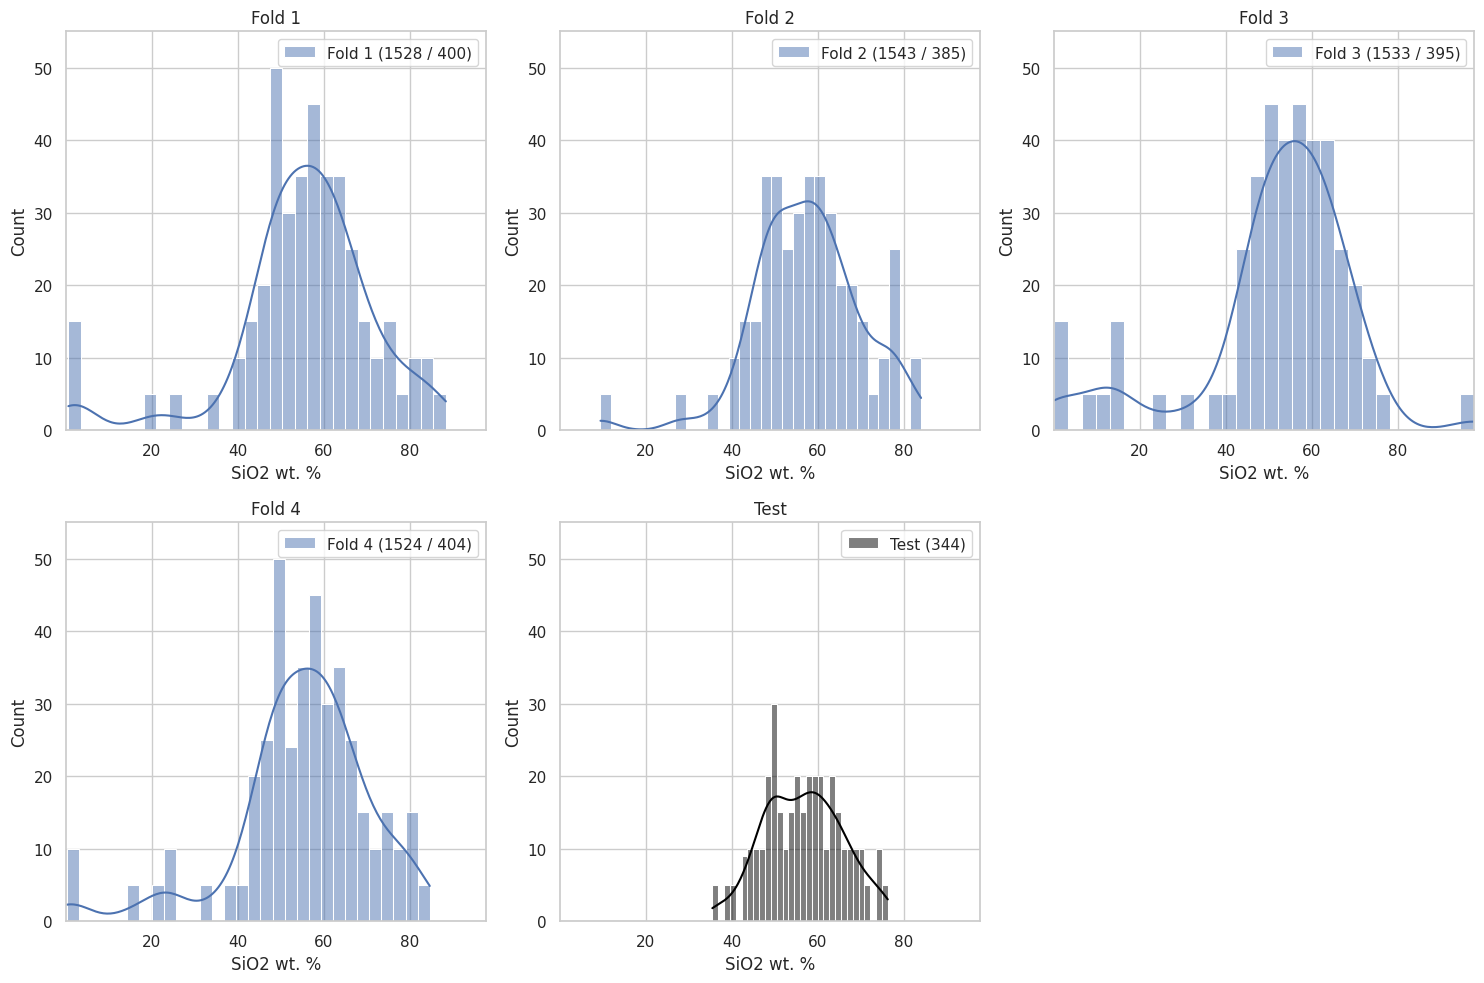
\includegraphics[width=\textwidth]{images/histogram_grid_plot.png}
    \caption{Histogram and \gls{kde} of \ce{SiO_2} Distribution in Each Fold. The y-axis represents the count of samples per bin, and the x-axis represents \ce{SiO_2} concentration. The notation in the legend indicates the amount of instances in the training/validation sets.}
    \label{fig:histogram_grid_plot}
\end{figure*}

\begin{figure*}[h!]
    \centering
    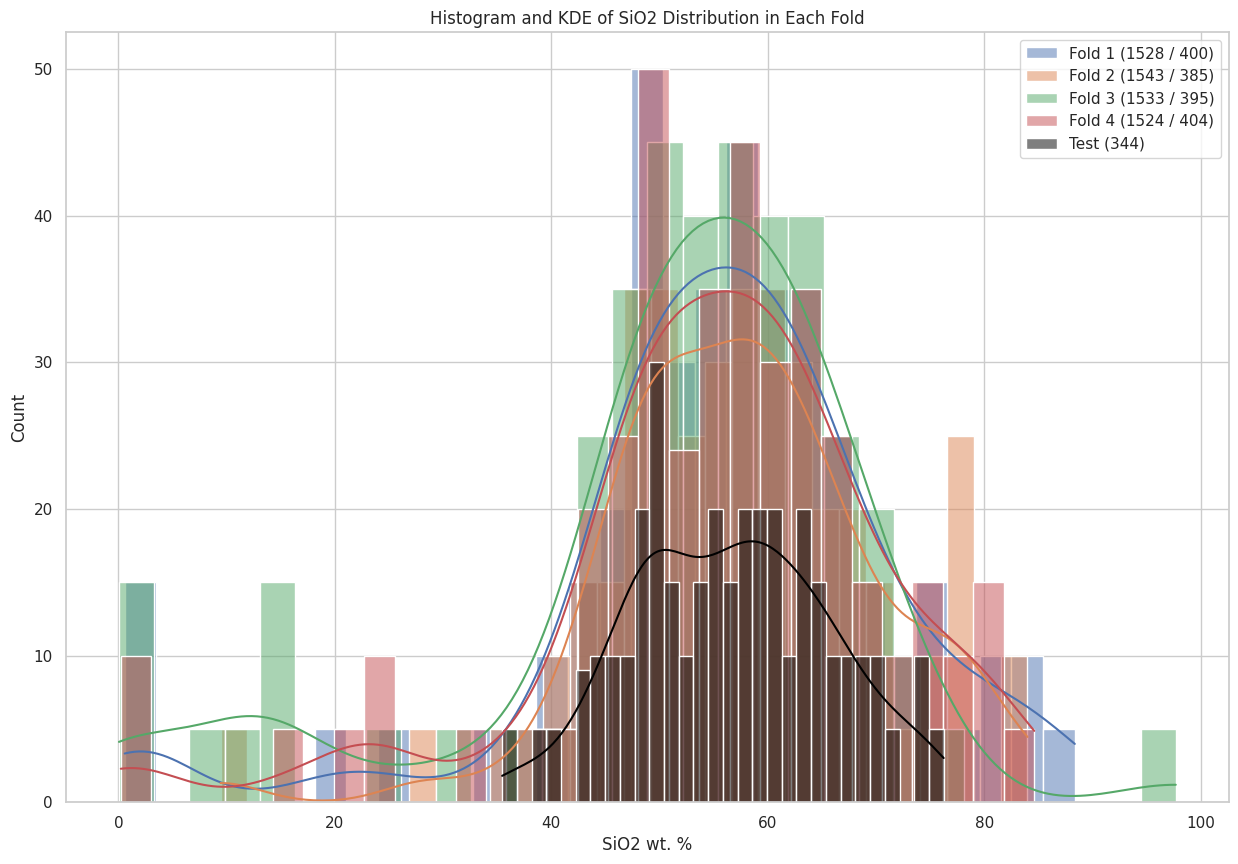
\includegraphics[width=\textwidth]{images/histogram_kde_plot.png}
    \caption{Combined Histogram and \gls{kde} of \ce{SiO_2} Distribution in Each Fold. The y-axis represents the count of samples per bin, and the x-axis represents \ce{SiO_2} concentration. The notation in the legend indicates the amount of instances in the training/validation sets.}
    \label{fig:histogram_kde_plot}
\end{figure*}

\begin{figure*}[h!]
    \centering
    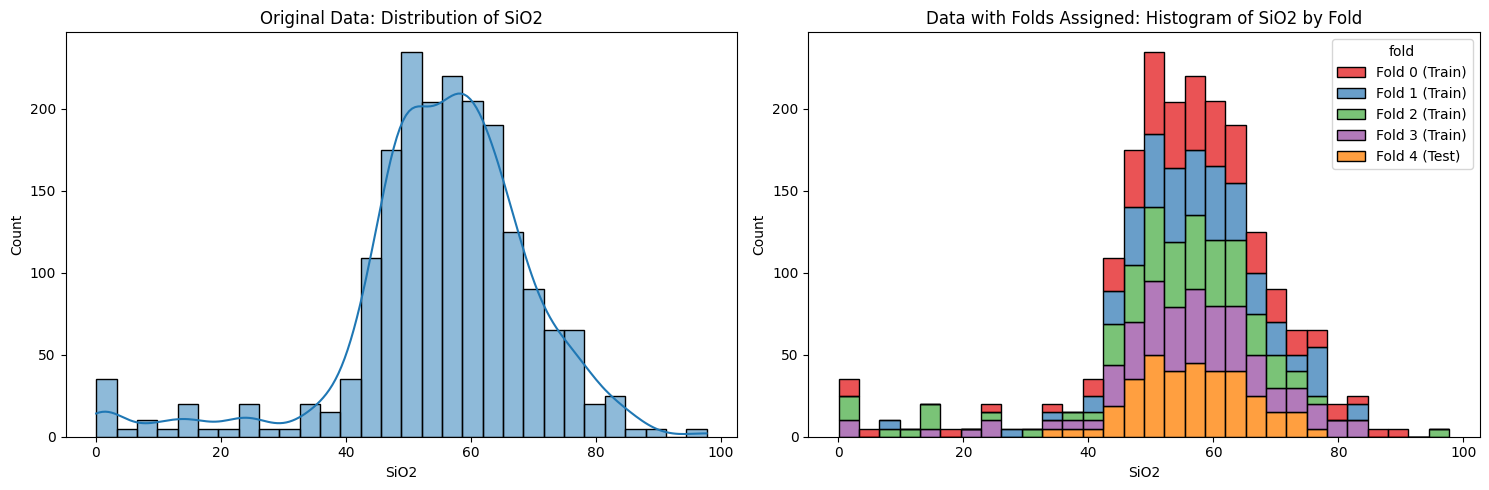
\includegraphics[width=\textwidth]{images/original_and_post_fold.png}
    \caption{Distribution of \ce{SiO_2} concentrations before and after fold assignment. The left plot shows the original distribution of \ce{SiO_2}, while the right plot shows the distribution with folds assigned, color-coded to indicate the different folds.}
    \label{fig:original_and_post_fold_plot}
\end{figure*}


To further validate our visual analysis, we can look at quantitative measures such as the means and standard deviations of \ce{SiO_2} concentrations across the folds and the overall dataset.

\begin{figure*}[htbp]
    \centering
    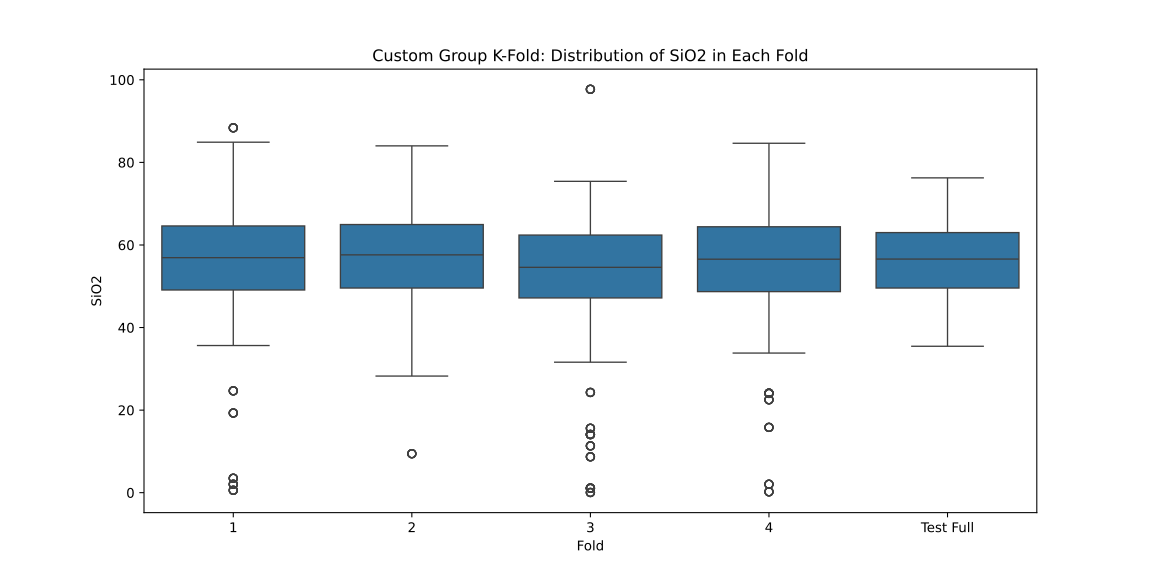
\includegraphics[width=\textwidth]{images/distribution_plot.png}
    \caption{Distribution of \ce{SiO_2} concentrations across cross-validation folds, training set, test set, and the entire dataset. The mean and standard deviation statistics for each partition are indicated figure.}
    \label{fig:siO2_distribution}
\end{figure*}

From Figure~\ref{fig:siO2_distribution}, it is evident that the means and standard deviations of \ce{SiO_2} concentrations for each fold, as well as the combined training set, are consistent with those of the full dataset.
This quantitative consistency supports the visual evidence that each training fold is representative of the entire dataset.
Furthermore, we can see that the standard deviation in the training sets is higher than the standard deviation in the test set, which is expected given the reassignment of extreme values to the training sets.

In conclusion, the visual and statistical analyses presented in this section confirm that our customized k-fold data partitioning procedure effectively maintains balanced and representative distributions across all folds.
This consistency is crucial for the robustness and generalizability of our models, as discussed in Section~\ref{subsec:validation_testing_procedures}.
The alignment between the visual evidence and the quantitative measures reinforces the reliability of our approach, ensuring that our models are well-equipped to perform accurately on unseen data.
\subsection{Design for Initial Experiment}\label{sec:initial-experiment}
As described in Section~\ref{sec:proposed_approach}, we conducted a series of initial experiments to evaluate the performance of various machine learning models on the prediction of major oxide compositions from our \gls{libs} dataset.
These experiments aimed to provide a preliminary assessment of the models' performance, allowing us to identify the most promising models for further evaluation and inclusion in our stacking ensemble.
All models were trained on the same preprocessed data using the Norm 3 preprocessing method described in Section~\ref{sec:norm3}.
This ensured that the models' performance could be evaluated under consistent and comparable conditions.

All models were trained using our data partitioning and cross-validation strategy, as described in Section~\ref{subsec:validation_testing_procedures}. 
To ensure as fair of a comparison between models as possible, all models were trained using as many default hyperparameters as possible, and those hyperparameters that did not have default options were selected based on values found in the literature.
However, due to the nature of the neural network models' architecture, some extra time was spent on tuning the models to ensure a fair comparison.
This included using batch normalization for the \gls{cnn} model, as early assesments showed that this was necessary to produce reasonable results.
Finally, we evaluated each model once per oxide given the selected configuration of hyperparameters. 
As stated, the goal of this experiment was merely to get an initial indication of the performance of the models.

The hyperparameters used for the models in the initial experiment can be found in the Appendix~\ref{subsec:initial_experiment_hyperparameters}.
\subsection{Initial Results}
Table~\ref{tab:init_results} presents the results of the initial experiments, including the \gls{rmsep}, \gls{rmsecv}, standard deviation, and standard deviation of cross-validation prediction errors for each model across all oxides.
The means of each metric are also provided to give an overall indication of the models' performance.
Furthermore, we present an overview of these mean values in Figure~\ref{fig:init_results_rmses} to facilitate a visual comparison of the models' general performance.

The results indicate that the gradient boosting models, \gls{xgboost}, \gls{gbr}, and \gls{ngboost}, consistently perform well across all oxides, with \gls{xgboost} generally outperforming the other two gradient boosting models.
Interestingly, \gls{gbr} has the lowest \gls{rmsep}, while \gls{xgboost} achieves the lowest \gls{rmsecv}, suggesting that the regularization in \gls{xgboost} may improve the model's generalizability.
These models exhibit both low mean \gls{rmsep} and \gls{rmsecv} values, indicating high accuracy, as well as low standard deviation values, underscoring their robustness.
\gls{svr} is also among the top-performing models, with mean \gls{rmsep} and \gls{rmsecv} values close to those of \gls{xgboost} and low standard deviation values.

While usually outperformed by gradient boosting models and \gls{svr}, the other ensemble models, \gls{rf} and \gls{etr}, also exhibit good performance.
The \gls{pls}, ridge, \gls{lasso}, and \gls{enet} models typically seem to perform worse than the other models, with higher mean \gls{rmsep} and \gls{rmsecv} values and higher standard deviation values.
We observe that \gls{enet} performs between ridge and \gls{lasso} in terms of both error and standard deviation, which aligns with expectations since \gls{enet} combines the regularization techniques of both models.

The \gls{cnn} and \gls{ann} models perform the worst across all oxides, exhibiting the highest mean \gls{rmsep} and \gls{rmsecv} values, as well as the highest standard deviation values.
This poor performance is further highlighted in Table~\ref{tab:relative_performance}, which shows the relative performance of each model compared to the best-performing model, \gls{xgboost}.
The table also includes the difference in performance relative to the next best model, with \gls{xgboost} serving as the baseline for comparison, assigned a relative performance of 100\%.
From this table, it is evident that the \gls{cnn} and \gls{ann} models experience notable drops in performance compared to the top-performing models.
While deep learning models such as these have the theoretical potential to perform well with \gls{libs} data, given their ability to learn complex patterns and relationships, the relatively small size of our dataset may limit their efficacy.
Furthermore, achieving optimal performance with these models necessitates extensive tuning of both their architectures and hyperparameters, which involves exploring a vast space of potential configurations and design choices.
Although methods for systematic hyperparameter optimization, as detailed in Section~\ref{sec:optimization_framework}, could be employed, the associated computational cost would be prohibitively high.
Additionally, there are numerous architectural design decisions and advanced techniques that could potentially enhance model performance, but their inclusion would expand the scope of this study beyond feasible limits.
For these reasons, we decided to exclude the \gls{cnn} and \gls{ann} models from further experimentation.

Tables~\ref{tab:best_results} and \ref{tab:best_model_occurrences} list the best-performing model for each oxide and the frequency with which each model achieves top performance according to various metrics, respectively.
These tables are intended to provide an overview of model performance rather than to determine an overall 'winner by majority'.
Their purpose is to illustrate the general trends and behavior of different models across various metrics and oxides.
Although \gls{xgboost} and \gls{svr} appear the most frequently in Table~\ref{tab:best_model_occurrences}, this does not imply that they are the best models for every oxide.
For example, if one were to only consider the mean of the performance metrics, \gls{pls} would be considered among the worst performing models, as shown in Figure~\ref{fig:init_results_rmses}.
However, inspecting Table~\ref{tab:best_results} reveals that \gls{pls} exhibits the lowest \gls{rmsecv} and standard deviation of prediction errors for both \ce{MgO} and \ce{Na2O}.
This indicates that \gls{pls} is the most accurate and robust model for these oxides, underscoring the importance of evaluating model performance on a per-oxide basis, as discussed in Section~\ref{sec:proposed_approach}.
Moreover, for some oxides, multiple models perform similarly well, such as \gls{xgboost}, \gls{gbr}, and ridge for \ce{CaO}.
This observation suggests the potential benefit of leveraging the strengths of multiple models, provided they do not make similar types of errors, which warrants further investigation.

To summarize, the initial results indicate that gradient boosting models, particularly \gls{xgboost}, demonstrated the most consistent and accurate performance across all oxides.
\gls{svr} also performed well, with similar accuracy and robustness to the gradient boosting models.
In contrast, deep learning models such as \gls{cnn} and \gls{ann} underperformed, likely due to the small dataset size and insufficient tuning of their architectures and hyperparameters.
Inspecting the model performances per oxide revealed that the best model varied depending on the oxide, and several models performed well for each oxide.
This emphasizes the need for further evaluation of model performances on a per-oxide basis to identify suitable configurations for our stacking ensemble approach, which aims to leverage the strengths of multiple models.

\begin{figure*}
    \centering
    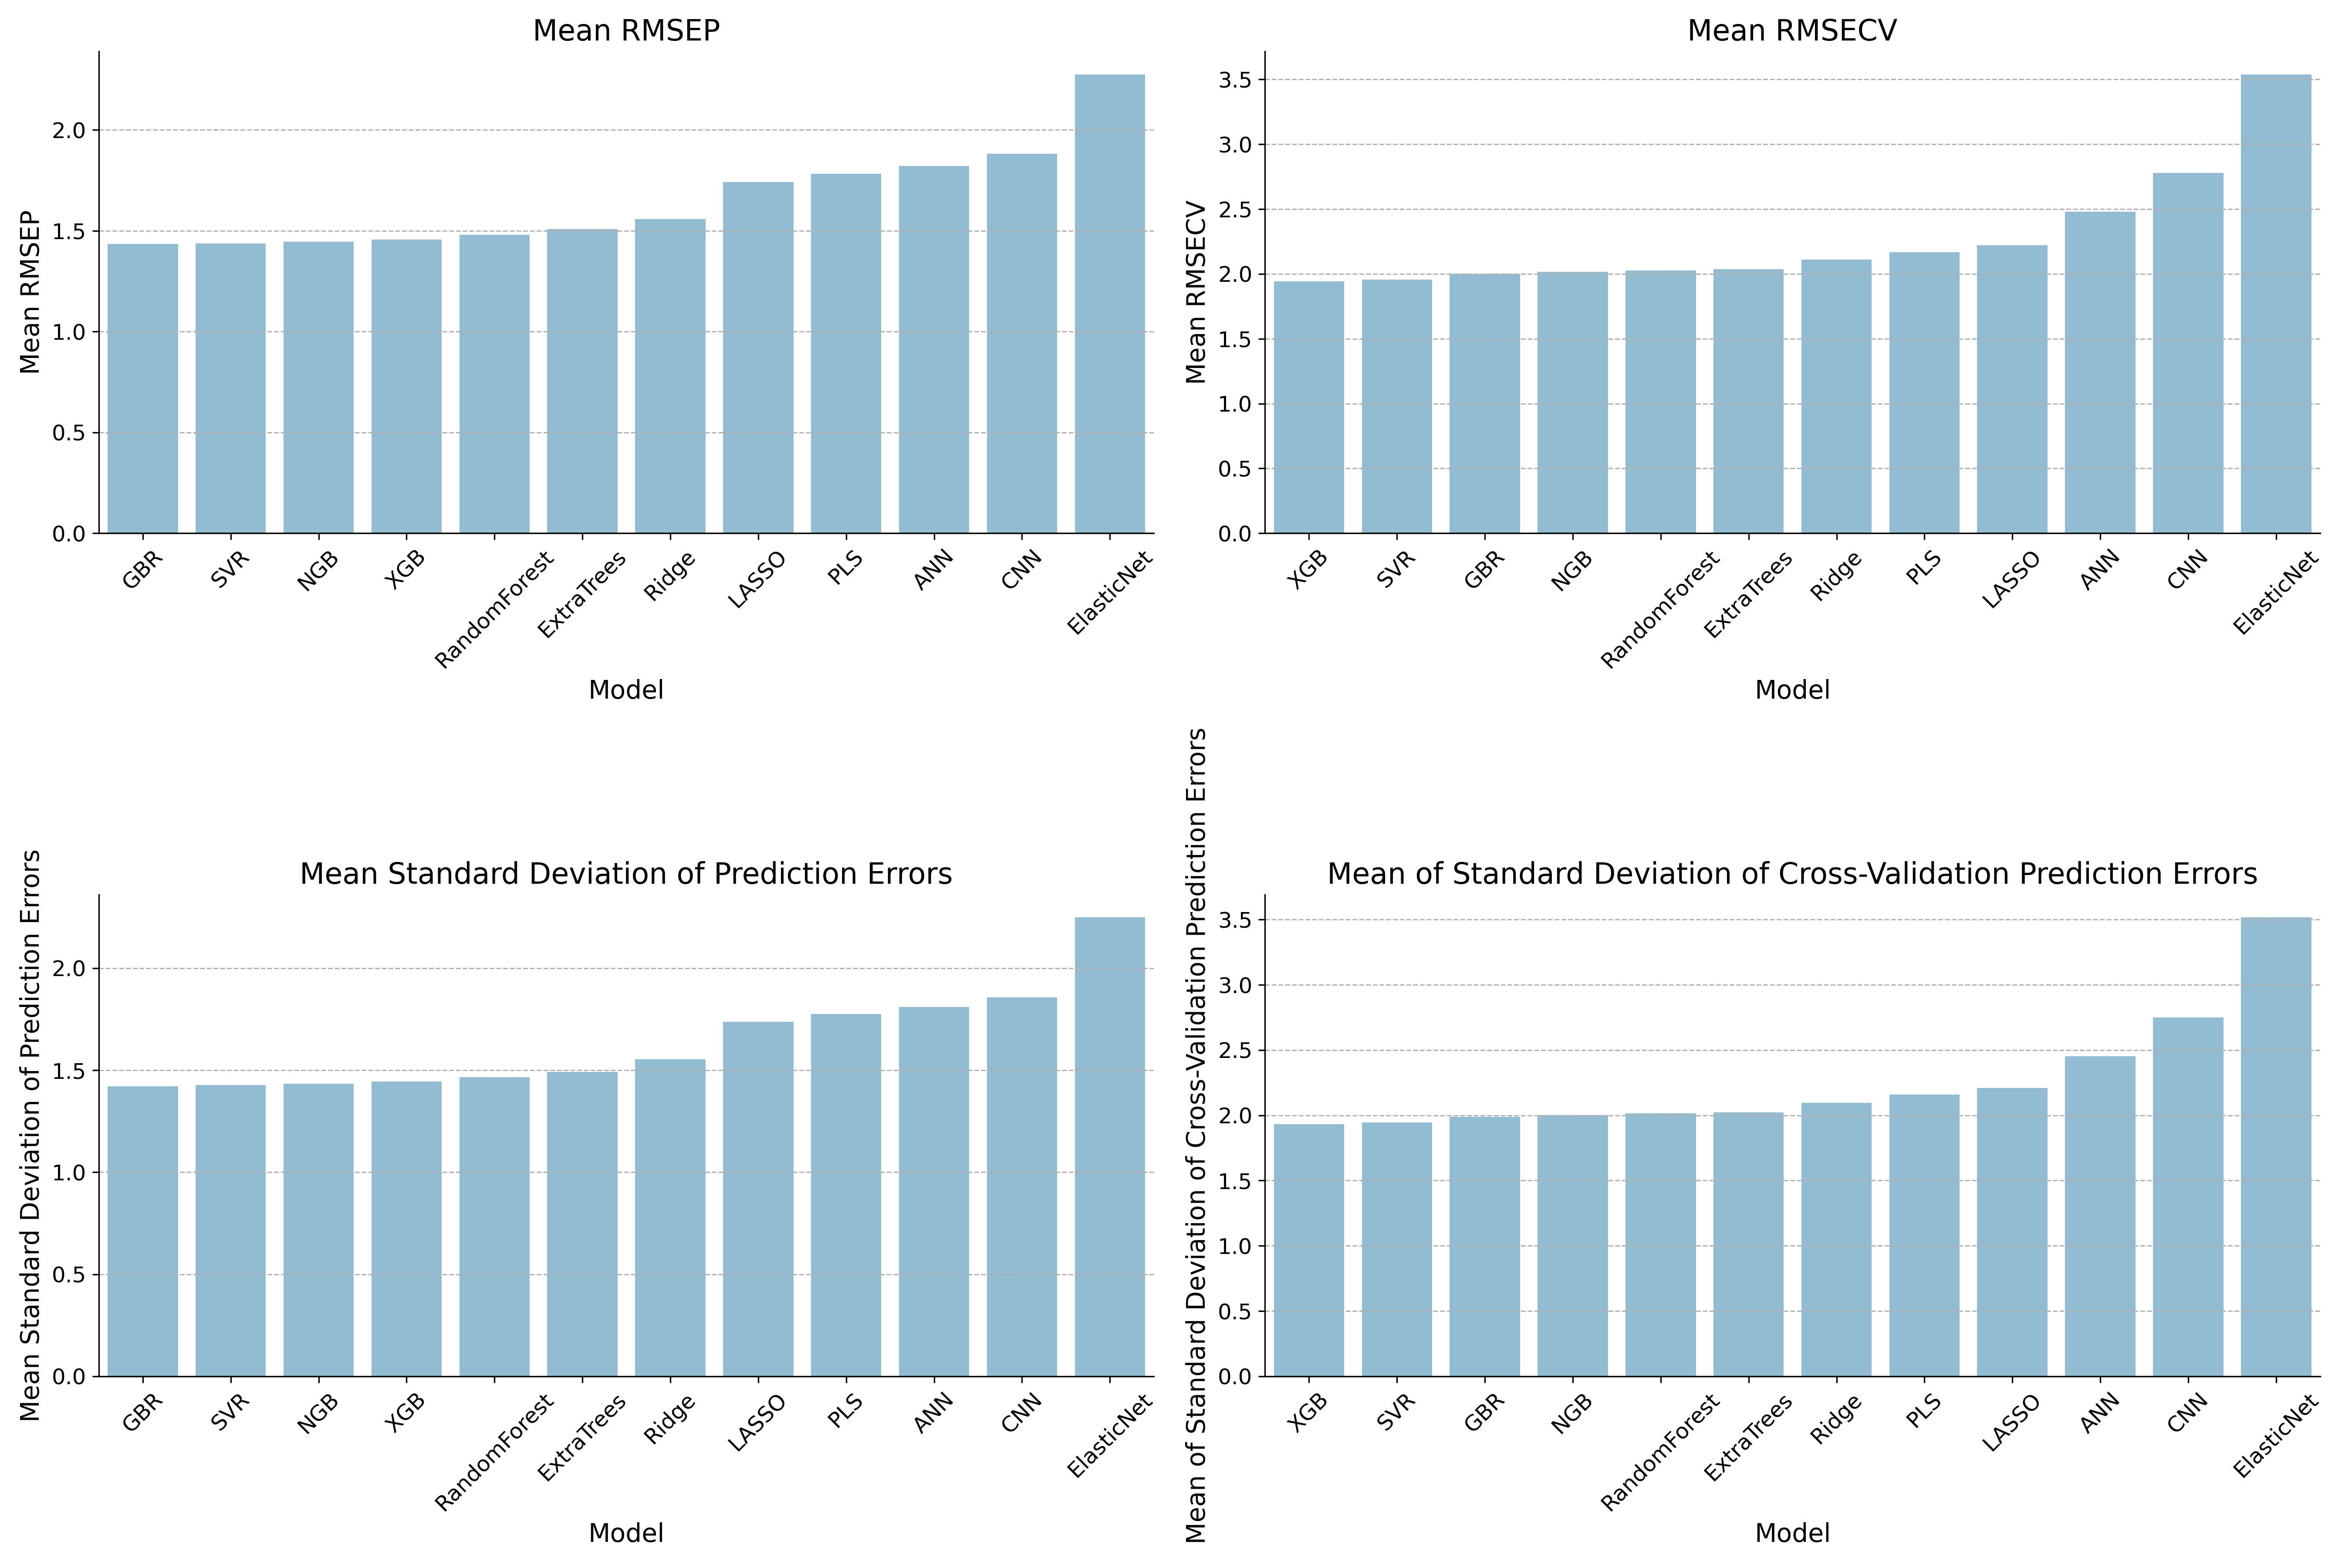
\includegraphics[width=\textwidth]{images/init_results_means.png}
    \caption{Mean \gls{rmsep}, \gls{rmsecv}, standard deviation of prediction errors, and standard deviation of cross-validation prediction errors for each model across all oxides.}
    \label{fig:init_results_rmses}
\end{figure*}

\begin{table}
\caption{Relative performance of each model compared to the best performing model, measured by normalized RMSECV and multiplied by 100 for percentage. A higher percentage indicates worse performance. The 'Diff. vs Prev.' column shows the difference in performance compared to the next best model, measured in percentage points.}
\begin{tabular}{lrr}
\toprule
Model & Relative Performance (\%) & Diff. vs Prev. \\
\midrule
XGB & 100.00 & - \\
SVR & 100.85 & 0.85 \\
GBR & 103.07 & 2.22 \\
NGB & 103.94 & 0.87 \\
RandomForest & 104.45 & 0.51 \\
ExtraTrees & 104.84 & 0.39 \\
Ridge & 105.04 & 0.20 \\
PLS & 111.66 & 6.61 \\
ElasticNet & 114.12 & 2.46 \\
LASSO & 114.30 & 0.19 \\
ANN & 127.82 & 13.52 \\
CNN & 143.18 & 15.36 \\
\bottomrule
\end{tabular}
\label{tab:relative_performance}
\end{table}

\begin{table*}[]
\centering
\caption{Initial results for the different models and metrics.}
\resizebox{1\textwidth}{!}{%
\begin{tabular}{l|cccc|cccc|cccc}
Model & \multicolumn{4}{c}{Ridge} & \multicolumn{4}{c}{\gls{lasso}} & \multicolumn{4}{c}{\gls{enet}} \\
Metric & \multicolumn{1}{c}{RMSEP} & \multicolumn{1}{c}{RMSECV} & \multicolumn{1}{c}{Std. dev.} & \multicolumn{1}{c}{Std. dev. CV} & \multicolumn{1}{c}{RMSEP} & \multicolumn{1}{c}{RMSECV} & \multicolumn{1}{c}{Std. dev.} & \multicolumn{1}{c}{Std. dev. CV} & \multicolumn{1}{c}{RMSEP} & \multicolumn{1}{c}{RMSECV} & \multicolumn{1}{c}{Std. dev.} & \multicolumn{1}{c}{Std. dev. CV} \\
\hline
$\ce{SiO2}$ & 4.104 & 5.004 & 4.108 & 5.005 & 4.412 & 5.431 & 4.417 & 5.437 & 4.412 & 5.431 & 4.417 & 5.437 \\
$\ce{TiO2}$ & 0.424 & 0.470 & 0.413 & 0.469 & 0.398 & 0.556 & 0.389 & 0.555 & 0.398 & 0.556 & 0.389 & 0.555 \\
$\ce{Al2O3}$ & 2.322 & 2.913 & 2.324 & 2.888 & 2.349 & 3.063 & 2.352 & 3.044 & 2.349 & 3.063 & 2.352 & 3.044 \\
$\ce{FeOT}$ & 2.068 & 3.173 & 2.070 & 3.122 & 2.236 & 3.490 & 2.238 & 3.440 & 2.236 & 3.490 & 2.238 & 3.440 \\
$\ce{MgO}$ & 1.150 & 1.509 & 1.152 & 1.492 & 1.267 & 1.682 & 1.249 & 1.661 & 1.267 & 1.682 & 1.249 & 1.661 \\
$\ce{CaO}$ & 1.844 & 1.485 & 1.833 & 1.478 & 1.963 & 1.554 & 1.962 & 1.549 & 1.963 & 1.554 & 1.962 & 1.549 \\
$\ce{Na2O}$ & 0.632 & 1.089 & 0.633 & 1.084 & 0.625 & 1.114 & 0.616 & 1.111 & 0.588 & 1.085 & 0.587 & 1.082 \\
$\ce{K2O}$ & 0.651 & 0.668 & 0.645 & 0.668 & 0.638 & 0.859 & 0.629 & 0.856 & 0.638 & 0.859 & 0.629 & 0.856 \\
\hline
Mean & 1.649 & 2.039 & 1.647 & 2.026 & 1.736 & 2.219 & 1.732 & 2.207 & 1.731 & 2.215 & 1.728 & 2.203 \\
\hline
Model & \multicolumn{4}{c}{\gls{pls}} & \multicolumn{4}{c}{\gls{svr}} & \multicolumn{4}{c}{\gls{rf}} \\
Metric & \multicolumn{1}{c}{RMSEP} & \multicolumn{1}{c}{RMSECV} & \multicolumn{1}{c}{Std. dev.} & \multicolumn{1}{c}{Std. dev. CV} & \multicolumn{1}{c}{RMSEP} & \multicolumn{1}{c}{RMSECV} & \multicolumn{1}{c}{Std. dev.} & \multicolumn{1}{c}{Std. dev. CV} & \multicolumn{1}{c}{RMSEP} & \multicolumn{1}{c}{RMSECV} & \multicolumn{1}{c}{Std. dev.} & \multicolumn{1}{c}{Std. dev. CV} \\
\hline
$\ce{SiO2}$ & 4.141 & 5.701 & 4.145 & 5.693 & 3.552 & 4.908 & 3.555 & 4.908 & 3.715 & 5.304 & 3.699 & 5.292 \\
$\ce{TiO2}$ & 0.452 & 0.531 & 0.441 & 0.530 & 0.461 & 0.463 & 0.455 & 0.462 & 0.331 & 0.427 & 0.321 & 0.425 \\
$\ce{Al2O3}$ & 2.073 & 3.322 & 2.061 & 3.302 & 1.931 & 2.700 & 1.934 & 2.693 & 2.076 & 2.443 & 2.079 & 2.433 \\
$\ce{FeOT}$ & 3.222 & 3.117 & 3.221 & 3.114 & 1.823 & 2.847 & 1.814 & 2.809 & 2.091 & 3.091 & 2.073 & 3.053 \\
$\ce{MgO}$ & 1.106 & 1.296 & 1.103 & 1.296 & 0.789 & 1.426 & 0.785 & 1.419 & 0.911 & 1.742 & 0.904 & 1.731 \\
$\ce{CaO}$ & 1.937 & 1.813 & 1.923 & 1.792 & 1.626 & 1.532 & 1.594 & 1.508 & 1.765 & 1.503 & 1.754 & 1.499 \\
$\ce{Na2O}$ & 0.545 & 0.908 & 0.536 & 0.906 & 0.742 & 1.096 & 0.725 & 1.086 & 0.420 & 1.028 & 0.421 & 1.023 \\
$\ce{K2O}$ & 0.774 & 0.650 & 0.772 & 0.646 & 0.567 & 0.690 & 0.555 & 0.689 & 0.524 & 0.681 & 0.476 & 0.676 \\
\hline
Mean & 1.781 & 2.167 & 1.775 & 2.160 & 1.436 & 1.958 & 1.427 & 1.947 & 1.479 & 2.027 & 1.466 & 2.017 \\
\hline
Model & \multicolumn{4}{c}{\gls{ngboost}} & \multicolumn{4}{c}{\gls{gbr}} & \multicolumn{4}{c}{\gls{xgboost}} \\
Metric & \multicolumn{1}{c}{RMSEP} & \multicolumn{1}{c}{RMSECV} & \multicolumn{1}{c}{Std. dev.} & \multicolumn{1}{c}{Std. dev. CV} & \multicolumn{1}{c}{RMSEP} & \multicolumn{1}{c}{RMSECV} & \multicolumn{1}{c}{Std. dev.} & \multicolumn{1}{c}{Std. dev. CV} & \multicolumn{1}{c}{RMSEP} & \multicolumn{1}{c}{RMSECV} & \multicolumn{1}{c}{Std. dev.} & \multicolumn{1}{c}{Std. dev. CV} \\
\hline
$\ce{SiO2}$ & 4.112 & 5.071 & 4.081 & 5.010 & 3.576 & 4.995 & 3.479 & 4.922 & 3.953 & 4.898 & 3.926 & 4.876 \\
$\ce{TiO2}$ & 0.340 & 0.433 & 0.333 & 0.430 & 0.474 & 0.449 & 0.473 & 0.446 & 0.334 & 0.437 & 0.328 & 0.436 \\
$\ce{Al2O3}$ & 1.931 & 2.291 & 1.933 & 2.282 & 1.894 & 2.518 & 1.891 & 2.511 & 1.912 & 2.198 & 1.913 & 2.193 \\
$\ce{FeOT}$ & 1.588 & 3.561 & 1.590 & 3.530 & 1.594 & 3.069 & 1.596 & 3.068 & 1.848 & 3.020 & 1.838 & 3.002 \\
$\ce{MgO}$ & 0.849 & 1.578 & 0.845 & 1.574 & 0.964 & 1.766 & 0.960 & 1.763 & 0.905 & 1.781 & 0.901 & 1.771 \\
$\ce{CaO}$ & 1.740 & 1.610 & 1.723 & 1.602 & 1.768 & 1.468 & 1.769 & 1.468 & 1.765 & 1.467 & 1.749 & 1.457 \\
$\ce{Na2O}$ & 0.416 & 0.921 & 0.415 & 0.916 & 0.481 & 1.130 & 0.481 & 1.123 & 0.387 & 1.071 & 0.387 & 1.062 \\
$\ce{K2O}$ & 0.582 & 0.675 & 0.545 & 0.673 & 0.727 & 0.609 & 0.719 & 0.610 & 0.547 & 0.658 & 0.511 & 0.657 \\
\hline
Mean & 1.445 & 2.017 & 1.433 & 2.002 & 1.435 & 2.001 & 1.421 & 1.989 & 1.456 & 1.941 & 1.444 & 1.932 \\
\hline
Model & \multicolumn{4}{c}{\gls{etr}} & \multicolumn{4}{c}{\gls{ann}} & \multicolumn{4}{c}{\gls{cnn}} \\
Metric & \multicolumn{1}{c}{RMSEP} & \multicolumn{1}{c}{RMSECV} & \multicolumn{1}{c}{Std. dev.} & \multicolumn{1}{c}{Std. dev. CV} & \multicolumn{1}{c}{RMSEP} & \multicolumn{1}{c}{RMSECV} & \multicolumn{1}{c}{Std. dev.} & \multicolumn{1}{c}{Std. dev. CV} & \multicolumn{1}{c}{RMSEP} & \multicolumn{1}{c}{RMSECV} & \multicolumn{1}{c}{Std. dev.} & \multicolumn{1}{c}{Std. dev. CV} \\
\hline
$\ce{SiO2}$ & 3.995 & 5.230 & 3.970 & 5.225 & 4.664 & 7.025 & 4.670 & 6.981 & 4.662 & 6.061 & 4.626 & 6.046 \\
$\ce{TiO2}$ & 0.330 & 0.439 & 0.321 & 0.438 & 0.436 & 0.543 & 0.431 & 0.540 & 0.571 & 0.634 & 0.565 & 0.628 \\
$\ce{Al2O3}$ & 1.845 & 2.368 & 1.847 & 2.359 & 2.624 & 3.049 & 2.628 & 3.026 & 2.482 & 2.871 & 2.457 & 2.854 \\
$\ce{FeOT}$ & 2.144 & 3.299 & 2.126 & 3.257 & 2.534 & 3.836 & 2.497 & 3.748 & 2.588 & 4.584 & 2.521 & 4.488 \\
$\ce{MgO}$ & 0.906 & 1.755 & 0.895 & 1.738 & 1.315 & 1.818 & 1.300 & 1.768 & 1.292 & 2.892 & 1.280 & 2.857 \\
$\ce{CaO}$ & 1.837 & 1.515 & 1.831 & 1.510 & 1.799 & 1.633 & 1.772 & 1.634 & 2.009 & 2.142 & 2.008 & 2.099 \\
$\ce{Na2O}$ & 0.411 & 1.031 & 0.409 & 1.028 & 0.539 & 1.095 & 0.532 & 1.091 & 0.656 & 1.364 & 0.657 & 1.357 \\
$\ce{K2O}$ & 0.591 & 0.642 & 0.540 & 0.636 & 0.659 & 0.850 & 0.640 & 0.845 & 0.783 & 1.684 & 0.742 & 1.657 \\
\hline
Mean & 1.507 & 2.035 & 1.492 & 2.024 & 1.821 & 2.481 & 1.809 & 2.454 & 1.880 & 2.779 & 1.857 & 2.748 \\
\hline
\end{tabular}%
}
\label{tab:init_results}
\end{table*}


\begin{table*}
\centering
\begin{minipage}{.7\textwidth}
  \centering
  \caption{Lowest metric and corresponding model for each oxide.}
  \begin{tabular}{l|llll}
Oxide & RMSEP & RMSECV & Std. dev. & Std. dev. CV \\
\hline
$\ce{SiO2}$ & 3.552 (\gls{svr}) & 4.898 (\gls{xgboost}) & 3.479 (\gls{gbr}) & 4.876 (\gls{xgboost}) \\
$\ce{TiO2}$ & 0.330 (\gls{etr}) & 0.427 (\gls{rf}) & 0.321 (\gls{etr}) & 0.425 (\gls{rf}) \\
$\ce{Al2O3}$ & 1.845 (\gls{etr}) & 2.198 (\gls{xgboost}) & 1.847 (\gls{etr}) & 2.193 (\gls{xgboost}) \\
$\ce{FeOT}$ & 1.588 (\gls{ngboost}) & 2.847 (\gls{svr}) & 1.590 (\gls{ngboost}) & 2.809 (\gls{svr}) \\
$\ce{MgO}$ & 0.789 (\gls{svr}) & 1.296 (\gls{pls}) & 0.785 (\gls{svr}) & 1.296 (\gls{pls}) \\
$\ce{CaO}$ & 1.626 (\gls{svr}) & 1.467 (\gls{xgboost}) & 1.594 (\gls{svr}) & 1.457 (\gls{xgboost}) \\
$\ce{Na2O}$ & 0.387 (\gls{xgboost}) & 0.908 (\gls{pls}) & 0.387 (\gls{xgboost}) & 0.906 (\gls{pls}) \\
$\ce{K2O}$ & 0.524 (\gls{rf}) & 0.609 (\gls{gbr}) & 0.476 (\gls{rf}) & 0.610 (\gls{gbr}) \\
\hline
\end{tabular}%
\label{tab:best_results}

  \label{tab:best_results}
\end{minipage}%
\hspace{0.03\textwidth}
\begin{minipage}{.25\textwidth}
  \centering
  \caption{Occurrences of the best model for each oxide.}
  \begin{table}[H]
\centering
\begin{tabular}{lc}
Model & Occurrences \\
\hline
\gls{xgboost} & 8 \\
\gls{svr} & 7 \\
\gls{etr} & 4 \\
\gls{rf} & 4 \\
\gls{pls} & 4 \\
\gls{gbr} & 3 \\
\gls{ngboost} & 2 \\
\end{tabular}
\caption{Occurrences of the best model for each oxide.}
\label{tab:best_model_occurrences}
\end{table}
\begin{tabular}{lc}
Model & Occurrences \\
\hline
\gls{xgboost} & 8 \\
\gls{svr} & 7 \\
\gls{etr} & 4 \\
\gls{rf} & 4 \\
\gls{pls} & 4 \\
\gls{gbr} & 3 \\
\gls{ngboost} & 2 \\
\end{tabular}
\label{tab:best_model_occurrences}

  \label{tab:best_model_occurrences}
\end{minipage}
\end{table*}

This section details the parameter ranges used for various preprocessing techniques and models in our Optuna optimization framework.
Our aim is to explore a wide range of preprocessing techniques and model combinations to identify the best-performing configurations for use in the stacking ensemble.

For preprocessing, we include a range of parameters for various transformers and scalars, as shown in Table~\ref{tab:optuna_model_configurations}.
The goal is to explore both conventionally used and novel preprocessing techniques with a wide range of parameters to maximize coverage while avoiding excessive search space expansion.
For instance, the number of components for \gls{pca} (1-50) and \gls{kernel-pca} (1-100) ensures essential feature capture while balancing computational load.
Flexibility is provided by including various categorical choices and numerical ranges, such as different kernel types in \gls{kernel-pca}, and logarithmic scales for gamma values ($10^{-3}$ to $10^{1}$), allowing models to adapt to diverse data characteristics.
Efficiency is maintained by using logarithmic scales for parameters that span several orders of magnitude, optimizing the search process.
Scaler parameters, such as the quantile ranges in \texttt{RobustScaler}, are designed to accommodate different data distributions.
Similarly, the transformation methods in \texttt{PowerTransformer} and \texttt{QuantileTransformer} are selected to handle a variety of data distributions.

\begin{table*}[h]
\centering
\begin{tabular}{@{}l>{\ttfamily}lp{0.5\textwidth}@{}}
\toprule
\textbf{Model}                       & \textbf{Parameter}                & \textbf{Range}                           \\ \midrule
\multirow{2}{*}{PCA}                 & n\_components                     & 1 - 50                                   \\ \cmidrule{2-3}
                                     & whiten                            & \{True, False\}                          \\ \midrule
\multirow{4}{*}{KernelPCA}           & n\_components                     & 1 - 100                                  \\ \cmidrule{2-3}
                                     & kernel                            & \{linear, poly, rbf, sigmoid, cosine\}   \\ \cmidrule{2-3}
                                     & gamma                             & $10^{-3}$ - $10^{1}$ (log scale)         \\ \cmidrule{2-3}
                                     & degree                            & 1 - 5                                    \\ \midrule
\multirow{2}{*}{RobustScaler}        & quantile\_range                   & \{25-75, 10-90, 5-95, 35-65, 30-70, 40-60\} \\ \cmidrule{2-3}
                                     & with\_centering                   & \{True, False\}                          \\ \midrule
\multirow{2}{*}{StandardScaler}      & with\_mean                        & \{True, False\}                          \\ \cmidrule{2-3}
                                     & with\_std                         & \{True, False\}                          \\ \midrule
MinMaxScaler                         & feature\_range                    & \{0,1\}, \{-1,1\}                        \\ \midrule
\multirow{2}{*}{PowerTransformer}    & method                            & yeo-johnson                              \\ \cmidrule{2-3}
                                     & standardize                       & \{True, False\}                          \\ \midrule
\multirow{3}{*}{QuantileTransformer} & n\_quantiles                      & 100 - 1000                               \\ \cmidrule{2-3}
                                     & output\_distribution              & \{uniform, normal\}                      \\ \cmidrule{2-3}
                                     & subsample                         & 10000 - 100000                           \\ \midrule
MaxAbsScaler                         & -                                 & -                                        \\ \midrule
Norm3Scaler                          & -                                 & -                                        \\ \midrule
\end{tabular}
\label{tab:optuna_model_configurations}
\caption{Optuna preprocessing configuration ranges.}
\end{table*}


For the models, we include a range of parameters for various regressors, as shown in Table~\ref{tab:optuna_model_configurations}.
Similar to the preprocessing parameters, we aim to cover a wide range of regressors and their respective hyperparameters while maintaining a balance between coverage and computational efficiency.
Parameters like the number of estimators for \gls{gbr} and \gls{xgboost} (100-1000) provide flexibility in controlling the model complexity and training duration.
The learning rate parameter, ranging from $10^{-3}$ to $10^{0}$ in logarithmic scale, allows fine-tuning of the model's convergence speed and accuracy.
Maximum depth settings for tree-based models (\gls{gbr}, \gls{xgboost}, \gls{rf}, and \gls{etr}) range from 2 to 15, ensuring sufficient depth to capture complex patterns while avoiding overfitting.
Moreover, the inclusion of different kernel types for \gls{svr} (linear, poly, rbf, sigmoid) and the use of logarithmic scales for parameters such as \texttt{C}, \texttt{epsilon}, and \texttt{gamma}, help in adapting the models to various data characteristics and distributions.
The parameter ranges are chosen to span multiple orders of magnitude, such as the regularization parameters \texttt{alpha} in \gls{lasso}, \gls{ridge}, and \gls{enet}, which range from $10^{-3}$ to $10^{3}$.


\begin{table*}[h]
\centering
\begin{tabular}{@{}l>{\ttfamily}lp{0.5\textwidth}@{}}
\toprule
\textbf{Model}                 & \textbf{Parameter}          & \textbf{Range}                           \\ \midrule
\multirow{5}{*}{\gls{gbr}}     & n\_estimators               & 100 - 1000                                \\ \cmidrule{2-3}
                               & learning\_rate              & $10^{-3}$ - $10^{0}$ (log scale)          \\ \cmidrule{2-3}
                               & max\_depth                  & 3 - 10                                    \\ \cmidrule{2-3}
                               & subsample                   & 0.5 - 1.0                                 \\ \cmidrule{2-3}
                               & max\_features               & \{sqrt, log2\}                            \\ \midrule
\multirow{6}{*}{\gls{svr}}     & C                           & $10^{-3}$ - $10^{3}$ (log scale)          \\ \cmidrule{2-3}
                               & epsilon                     & $10^{-3}$ - $10^{1}$ (log scale)          \\ \cmidrule{2-3}
                               & kernel                      & \{linear, poly, rbf, sigmoid\}            \\ \cmidrule{2-3}
                               & degree                      & 1 - 5                                     \\ \cmidrule{2-3}
                               & gamma                       & \{scale, auto\}                           \\ \cmidrule{2-3}
                               & coef0                       & 0 - 10                                    \\ \midrule
\multirow{8}{*}{\gls{xgboost}} & n\_estimators               & 100 - 1000                                \\ \cmidrule{2-3}
                               & learning\_rate              & $10^{-3}$ - $10^{0}$ (log scale)          \\ \cmidrule{2-3}
                               & max\_depth                  & 2 - 15                                    \\ \cmidrule{2-3}
                               & subsample                   & 0.3 - 1.0                                 \\ \cmidrule{2-3}
                               & colsample\_bytree           & 0.5 - 1.0                                 \\ \cmidrule{2-3}
                               & gamma                       & $10^{-3}$ - $10^{1}$ (log scale)          \\ \cmidrule{2-3}
                               & reg\_alpha                  & $10^{-3}$ - $10^{3}$ (log scale)          \\ \cmidrule{2-3}
                               & reg\_lambda                 & $10^{-3}$ - $10^{3}$ (log scale)          \\ \midrule
\multirow{5}{*}{\gls{etr}}     & n\_estimators               & 100 - 1000                                \\ \cmidrule{2-3}
                               & max\_depth                  & 2 - 15                                    \\ \cmidrule{2-3}
                               & min\_samples\_split         & 2 - 20                                    \\ \cmidrule{2-3}
                               & min\_samples\_leaf          & 1 - 25                                    \\ \cmidrule{2-3}
                               & max\_features               & \{sqrt, log2\}                            \\ \midrule
PLS                            & n\_components               & 1 - 30                                    \\ \midrule
\multirow{8}{*}{\gls{ngboost}} & max\_depth                  & 2 - 10                                    \\ \cmidrule{2-3}
                               & natural\_gradient           & \{True, False\}                           \\ \cmidrule{2-3}
                               & n\_estimators               & 50 - 1000                                 \\ \cmidrule{2-3}
                               & learning\_rate              & 0.01 - 0.5 (log scale)                    \\ \cmidrule{2-3}
                               & minibatch\_frac             & 0.5 - 1.0                                 \\ \cmidrule{2-3}
                               & col\_sample                 & 0.5 - 1.0                                 \\ \cmidrule{2-3}
                               & tol                         & $10^{-5}$ - $10^{-3}$ (log scale)         \\ \cmidrule{2-3}
                               & validation\_fraction        & 0.1 - 0.5                                 \\ \cmidrule{2-3}
                               & early\_stopping\_rounds     & 10 - 100                                  \\ \midrule
Lasso                          & alpha                       & $10^{-3}$ - $10^{3}$ (log scale)          \\ \midrule
Ridge                          & alpha                       & $10^{-3}$ - $10^{3}$ (log scale)          \\ \midrule
\multirow{2}{*}{\gls{enet}}    & alpha                       & $10^{-3}$ - $10^{3}$ (log scale)          \\ \cmidrule{2-3}
                               & l1\_ratio                   & 0 - 1                                     \\ \midrule
\multirow{5}{*}{\gls{rf}}      & n\_estimators               & 100 - 300                                 \\ \cmidrule{2-3}
                               & max\_depth                  & 2 - 15                                    \\ \cmidrule{2-3}
                               & min\_samples\_split         & 2 - 10                                    \\ \cmidrule{2-3}
                               & min\_samples\_leaf          & 1 - 10                                    \\ \cmidrule{2-3}
                               & max\_features               & \{sqrt, log2\}                            \\ \bottomrule
\end{tabular}
\label{tab:optuna_model_configurations}
\caption{Optuna model configuration ranges.}
\end{table*}
\subsection{Optimization Experiment Design}\label{subsec:optimization_experiment_design}
Using the remaining ten models, we conducted an extended experiment to further refine their performance for each oxide. 
The goal was to identify which preprocessing techniques and hyperparameters would yield the best performance for each model by doing a thorough search for each configuration. 
To achieve this, we evaluated multiple permutations of each model with various preprocessors and hyperparameter configurations. 
Each configuration included a mandatory scaler, while data transformation and dimensionality reduction techniques were optional. 
The optimization process was conducted using our optimization framework, outlined in Section~\ref{sec:optimization_framework}

To ensure a fair assessment of each configuration, we needed to balance conducting enough iterations for the optimization to converge with the practical limitations imposed by our time constraints.
Therefore, we decided to perform 200 iterations per model for each oxide, resulting in a total of 16,000 iterations across ten models and eight oxides.
We deemed this to be a reasonable number of iterations to obtain a reliable indication of the performance of each configuration.
As mentioned in Section~\ref{sec:optimization_framework}, we used the \gls{tpe} algorithm for the optimization process.
For this sampler, we set the number of startup trials to 25\%.
The number of startup trials determines the number of random samples drawn before the \gls{tpe} sampler engages.
By choosing 25\%, we would reserved the first quarter of the iterations for exploration.
We believed this approach would allow sufficient time for the sampler to explore the search space while still providing enough iterations for refinement.

For the experiment, we defined a range or set of discrete values for each hyperparameter of the models and preprocessors.
To determine these ranges, we used a combination of values reported in the literature, our own analysis, and the default values for each hyperparameter as a starting point.
Our methodology involved expanding the hyperparameters with value ranges to include reasonable lower and upper extremes.
For hyperparameters with a discrete set of possible values, we included all options. 
As an example, for the \gls{pls} model, we used the elbow method to approximate the optimal number of components. 
Based on this, we defined the lower extreme as 1 and the upper extreme as 30, as we believed that the optimal number of components would be somewhere within this range. 
A similar approach was used for the preprocessor \gls{kernel-pca}, where we defined the number of components to be between 1 and 100.

A different example is \gls{gbr}, which was based on the default values for the hyperparameters.
The default value for the number of estimators is 100, so we defined this to be the bottom of the range and 1000 as the upper extreme. 
Given the complexity of the patterns in \gls{libs} data, we believed that the ideal number of weak learners would likely be above 100, and therefore believed that 100 was a reasonable lower bound. 
Determining the upper bound was more difficult, but we believed that 1000 was a reasonable upper bound, as it would allow the model to sufficiently capture the patterns in the data. 
Given that we allow for a relatively large number of estimators, we wanted to balance this with a relatively low bound for the learning rate. 
We did this to ensure the search space included a learning rate that could scale with the number of estimators and reduce the likelihood of overfitting. 
The default value for the learning rate is 0.1, so we defined the lower bound to be $10^{-3}$ and the upper bound to be 1. 
The max depth of each weak learner was set between 3 and 10, allowing for varying levels of complexity depending on what is needed based on the number of estimators. 
The subsample parameter was set between 0.5 and 1.0, to accommodate random sampling of the data when fitting each weak learner. 
Finally, the max features parameter was set to either \textit{sqrt} or \textit{log2}. Since this parameter has a discrete set of possible values, we included all options.

Using this approach of considering reasonable lower and upper bounds for each hyperparameter or using all options for discrete hyperparameters, we defined the ranges for each model and preprocessor.

The selected hyperparameter ranges for each model and preprocessor can be found in Table~\ref{tab:optuna_model_configurations} and Table~\ref{tab:optuna_preprocessing_configurations}, respectively.



\subsection{Optimization Results}\label{sec:optimization_results}
In this section, we present and analyze the results of running the optimization experiment that we described in Section~\ref{subsec:optimization_experiment_design}.
As mentioned, our primary objective was to identify the optimal configurations for predicting the concentration of various oxides in our dataset.
We systematically evaluated a range of machine learning models, preprocessing techniques, and hyperparameter settings to determine the most effective combinations for each oxide.

The results of the experiment were ~$16.000$ trials worth of data on the configurations used, hyperparameters, as well as metrics.

Our data cleaning for this dataset primarily included filtering out failed runs, which was caused by configurations that did not work well together, as well as filtering out extreme error values.
We filter out any runs that had an \gls{rmsecv} above 50.
Approaches like \gls{svr} could occasionally yield this kind of outlier result in specific configurations.
We chose a threshold of 50 to include as many trials that were not clearly outliers.

Our experiment proceeded mostly without encountering any issues.
Some issues are to be expected given the scale of the experiment.
Unfortunately, we encountered an issue with a server we were using, resulting in some oxides and models having to be re-run.
We managed to recover and re-run most of these.
However, \gls{ngboost} for \ce{MgO} was only partially finished.
Given that each model of the ten models would undergo 200 trials, for each oxide, this resulted in 2000 runs per oxide.
The exception is \ce{MgO}, for which \gls{ngboost} ran 143 trials, making the total trials for \ce{MgO} 1943.
After the filtering process, we are left with a total of 15245 trials to analyze.

Since we stored the configurations as well as each hyperparameter value for the trials, we had \~100 variables to consider during our analysis.
Among these, the primary variables of interest are the metrics and overall configuration variables, namely \texttt{Model Type}, \texttt{Scaler Type}, \texttt{PCA Type}, and \texttt{Transformer Type}.

We used this data to identify the best configurations for each oxide, as measured by \gls{rmsecv}.
We began our analysis broadly by examining the usage of preprocessors across trials. Subsequently, we narrowed our focus and reviewed the top 100 trials for each oxide to identify the optimal model, scaler, and transformer for each oxide.
Finally, we examined the single best-performing configurations across oxides, showing one configuration per model for each oxide.

As described in Section~\ref{sec:optimization_framework}, our optimization system searches for the best configurations through multi-objective optimization.
The optimization process involves adjusting the configuration and hyperparameters of the machine learning model and preprocessing pipeline to minimize the objective.
As the sampler conducts initial exploration and subsequently seeks to identify the optimal configuration through exploitation, we expect that the values of variables frequently appearing in the results are most likely to be optimal.
Table \ref{tab:scalers_comparison}, \ref{tab:pca_comparison}, and \ref{tab:transformers_comparison} display these values for the various preprocessors.
The optimization results indicate that configurations with the highest total values across oxides are often the most frequently exploited, suggesting they are most likely to optimize performance.
\texttt{Norm3Scaler} was used in 5090 trials, and therefore appears to be the most effective scaler.
This outcome was expected, as the method was specifically designed for this type of \gls{libs} dataset, as discussed in Section~\ref{sec:norm3}.
For dimensionality reduction, we see that \texttt{None}, indicating no \gls{pca}, was used in 9419 trials, constituting approximately 59\% of all trials.
This suggests that either no dimensionality reduction is optimal, or a more suitable method should be identified.
Neither \gls{pca} nor \gls{kernel-pca} are very effective for this dataset.
\texttt{QuantileTransformer} was used in 5710 trials, indicating that it may be the most optimal transformer.
We observe that \texttt{PowerTransformer} was employed in 5277 trials, while no transformer was used in 4956 trials. Unlike other preprocessing method types, there does not appear to be a clear winner for the transformers.

\begin{table*}
    \centering
    \begin{tabular}{lccccccccc}
        \toprule
        \textbf{Oxide} & \texttt{MaxAbsScaler} & \texttt{MinMaxScaler} & \texttt{Norm3Scaler} & \texttt{RobustScaler} & \texttt{StandardScaler} \\
        \midrule
        \ce{Al2O3}               & 336  & 476  & 495  & 453  & 240 \\
        \ce{CaO}                 & 310  & 362  & 681  & 338  & 309 \\
        \ce{FeO_T}               & 498  & 287  & 561  & 339  & 315 \\
        \ce{K2O}                 & 258  & 320  & 622  & 430  & 370 \\
        \ce{MgO}                 & 239  & 340  & 646  & 413  & 305 \\
        \ce{Na2O}                & 316  & 327  & 748  & 320  & 289 \\
        \ce{SiO2}                & 221  & 421  & 830  & 309  & 219 \\
        \ce{TiO2}                & 280  & 322  & 507  & 565  & 326 \\
        Total across oxides      & 2458 & 2855 & 5090 & 3167 & 2373 \\
        \bottomrule
    \end{tabular}
    \caption{Comparison of different scalers across the eight major oxides.}
    \label{tab:scalers_comparison}
\end{table*}


\begin{table*}
    \centering
    \begin{tabular}{lccccccccc}
        \toprule
        \textbf{Oxide} & \texttt{None} & \texttt{KernelPCA} & \texttt{PCA} \\
        \midrule
        \ce{Al2O3}               & 1243  & 389  & 368 \\
        \ce{CaO}                 & 1246  & 374  & 380 \\
        \ce{FeO_T}               & 1217  & 382  & 401 \\
        \ce{K2O}                 & 1250  & 373  & 377 \\
        \ce{MgO}                 & 1037  & 543  & 363 \\
        \ce{Na2O}                & 1167  & 382  & 451 \\
        \ce{SiO2}                & 1096  & 457  & 447 \\
        \ce{TiO2}                & 1163  & 468  & 369 \\
        Total across oxides      & 9419  & 3368 & 3156 \\
        \bottomrule
    \end{tabular}
    \caption{Comparison of different PCA types across the eight major oxides.}
    \label{tab:pca_comparison}
\end{table*}


\begin{table*}
    \centering
    \begin{tabular}{lccccccccc}
        \toprule
        \textbf{Oxide} & \texttt{None} & \texttt{PowerTransformer} & \texttt{QuantileTransformer} \\
        \midrule
        \ce{Al2O3}               & 442  & 649  & 909 \\
        \ce{CaO}                 & 673  & 595  & 732 \\
        \ce{FeO_T}               & 633  & 644  & 723 \\
        \ce{K2O}                 & 504  & 822  & 674 \\
        \ce{MgO}                 & 725  & 701  & 517 \\
        \ce{Na2O}                & 441  & 583  & 976 \\
        \ce{SiO2}                & 760  & 566  & 674 \\
        \ce{TiO2}                & 778  & 717  & 505 \\
        Total across oxides      & 4956 & 5277 & 5710 \\
        \bottomrule
    \end{tabular}
    \caption{Comparison of different transformers across the eight major oxides.}
    \label{tab:transformers_comparison}
\end{table*}

We chose to examine the top 100 trials for each configuration to provide a clearer understanding of the performance variance among the best configurations.
Given the wide range of configurations and their varying sensitivity to tuning, data distributions, and other factors, examining all trials would result in misleading descriptive statistics.
By focusing on the top 100 trials, we can more accurately identify which configurations perform well.
While a quantitative analysis of the top 10\% of trials based on metrics like \gls{rmsecv}, \gls{rmsep}, and other factors was feasible, selecting the top 100 trials for each oxide made it easier to see how many trials were present for each oxide.
This approach helps us avoid the 'best of the worst' scenario and ensures that we are analyzing a representative set of good configurations.
We present the results in Figure~\ref{fig:top100_models}, \ref{fig:top100_scalers}, \ref{fig:top100_transformers}, and \ref{fig:top100_pca}.
These figures and their corresponding subplots illustrate the performance of various configuration elements (models, scalers, transformers, PCA techniques) for each oxide, based on their \gls{rmsecv}.
Any elements that do not appear in a subplot were not used in the top 100 trials for the given oxide.
It is important to note that the variance in performance is influenced by multiple factors, not solely by the variable depicted in each plot.
Factors such as the interaction between different preprocessing techniques, specific hyperparameter settings, and the inherent variability in the data all contribute to the observed performance.
Therefore, while the plots offer valuable insights into the effectiveness of individual configuration elements, the overall performance is a result of complex interactions within the entire machine learning pipeline.
Therefore, we prioritize the analysis of the top-performing trials and examine a larger sample of these to draw generalizable conclusions about the optimal configurations for each oxide.

From Figure~\ref{fig:top100_models}, it is evident that \gls{svr}, gradient boosting methods, and \gls{pls} demonstrate the best performance.
Figure~\ref{fig:top100_pca} confirms our earlier hypothesis that not using any \gls{pca} or \gls{kernel-pca} yields the lowest \gls{rmsecv} values.
However, we do observe that either \gls{pca} or \gls{kernel-pca} appear in four of the plots, with \gls{kernel-pca} being the most frequently used among them.
This indicates that they are indeed used in some of the top-performing configurations.
Interestingly, Figure~\ref{fig:top100_scalers} shows that, although \texttt{Norm3Scaler} is the most frequently used and best-performing scaler, this is not always the case.
Min-max scaling appears to yield better results for \ce{SiO2} and \ce{CaO}, while robust scaling seems more effective for \ce{MgO}.
For \ce{Al2O3}, Norm 3 scaling exhibits the lowest \gls{rmsecv} values but a higher mean \gls{rmsecv} value compared to the other scalers.
Finally, Figure~\ref{fig:top100_transformers} reveals another nuanced finding.
Power transformations appear to most frequently yield the best results across oxides, while quantile transformation or no transformation show the lowest \gls{rmsecv} values for the remaining oxides.

These results further reinforce our hypothesis that a tailored configuration is necessary for each oxide, and there is no single configuration that performs well across all oxides.

\begin{figure*}
    \centering
    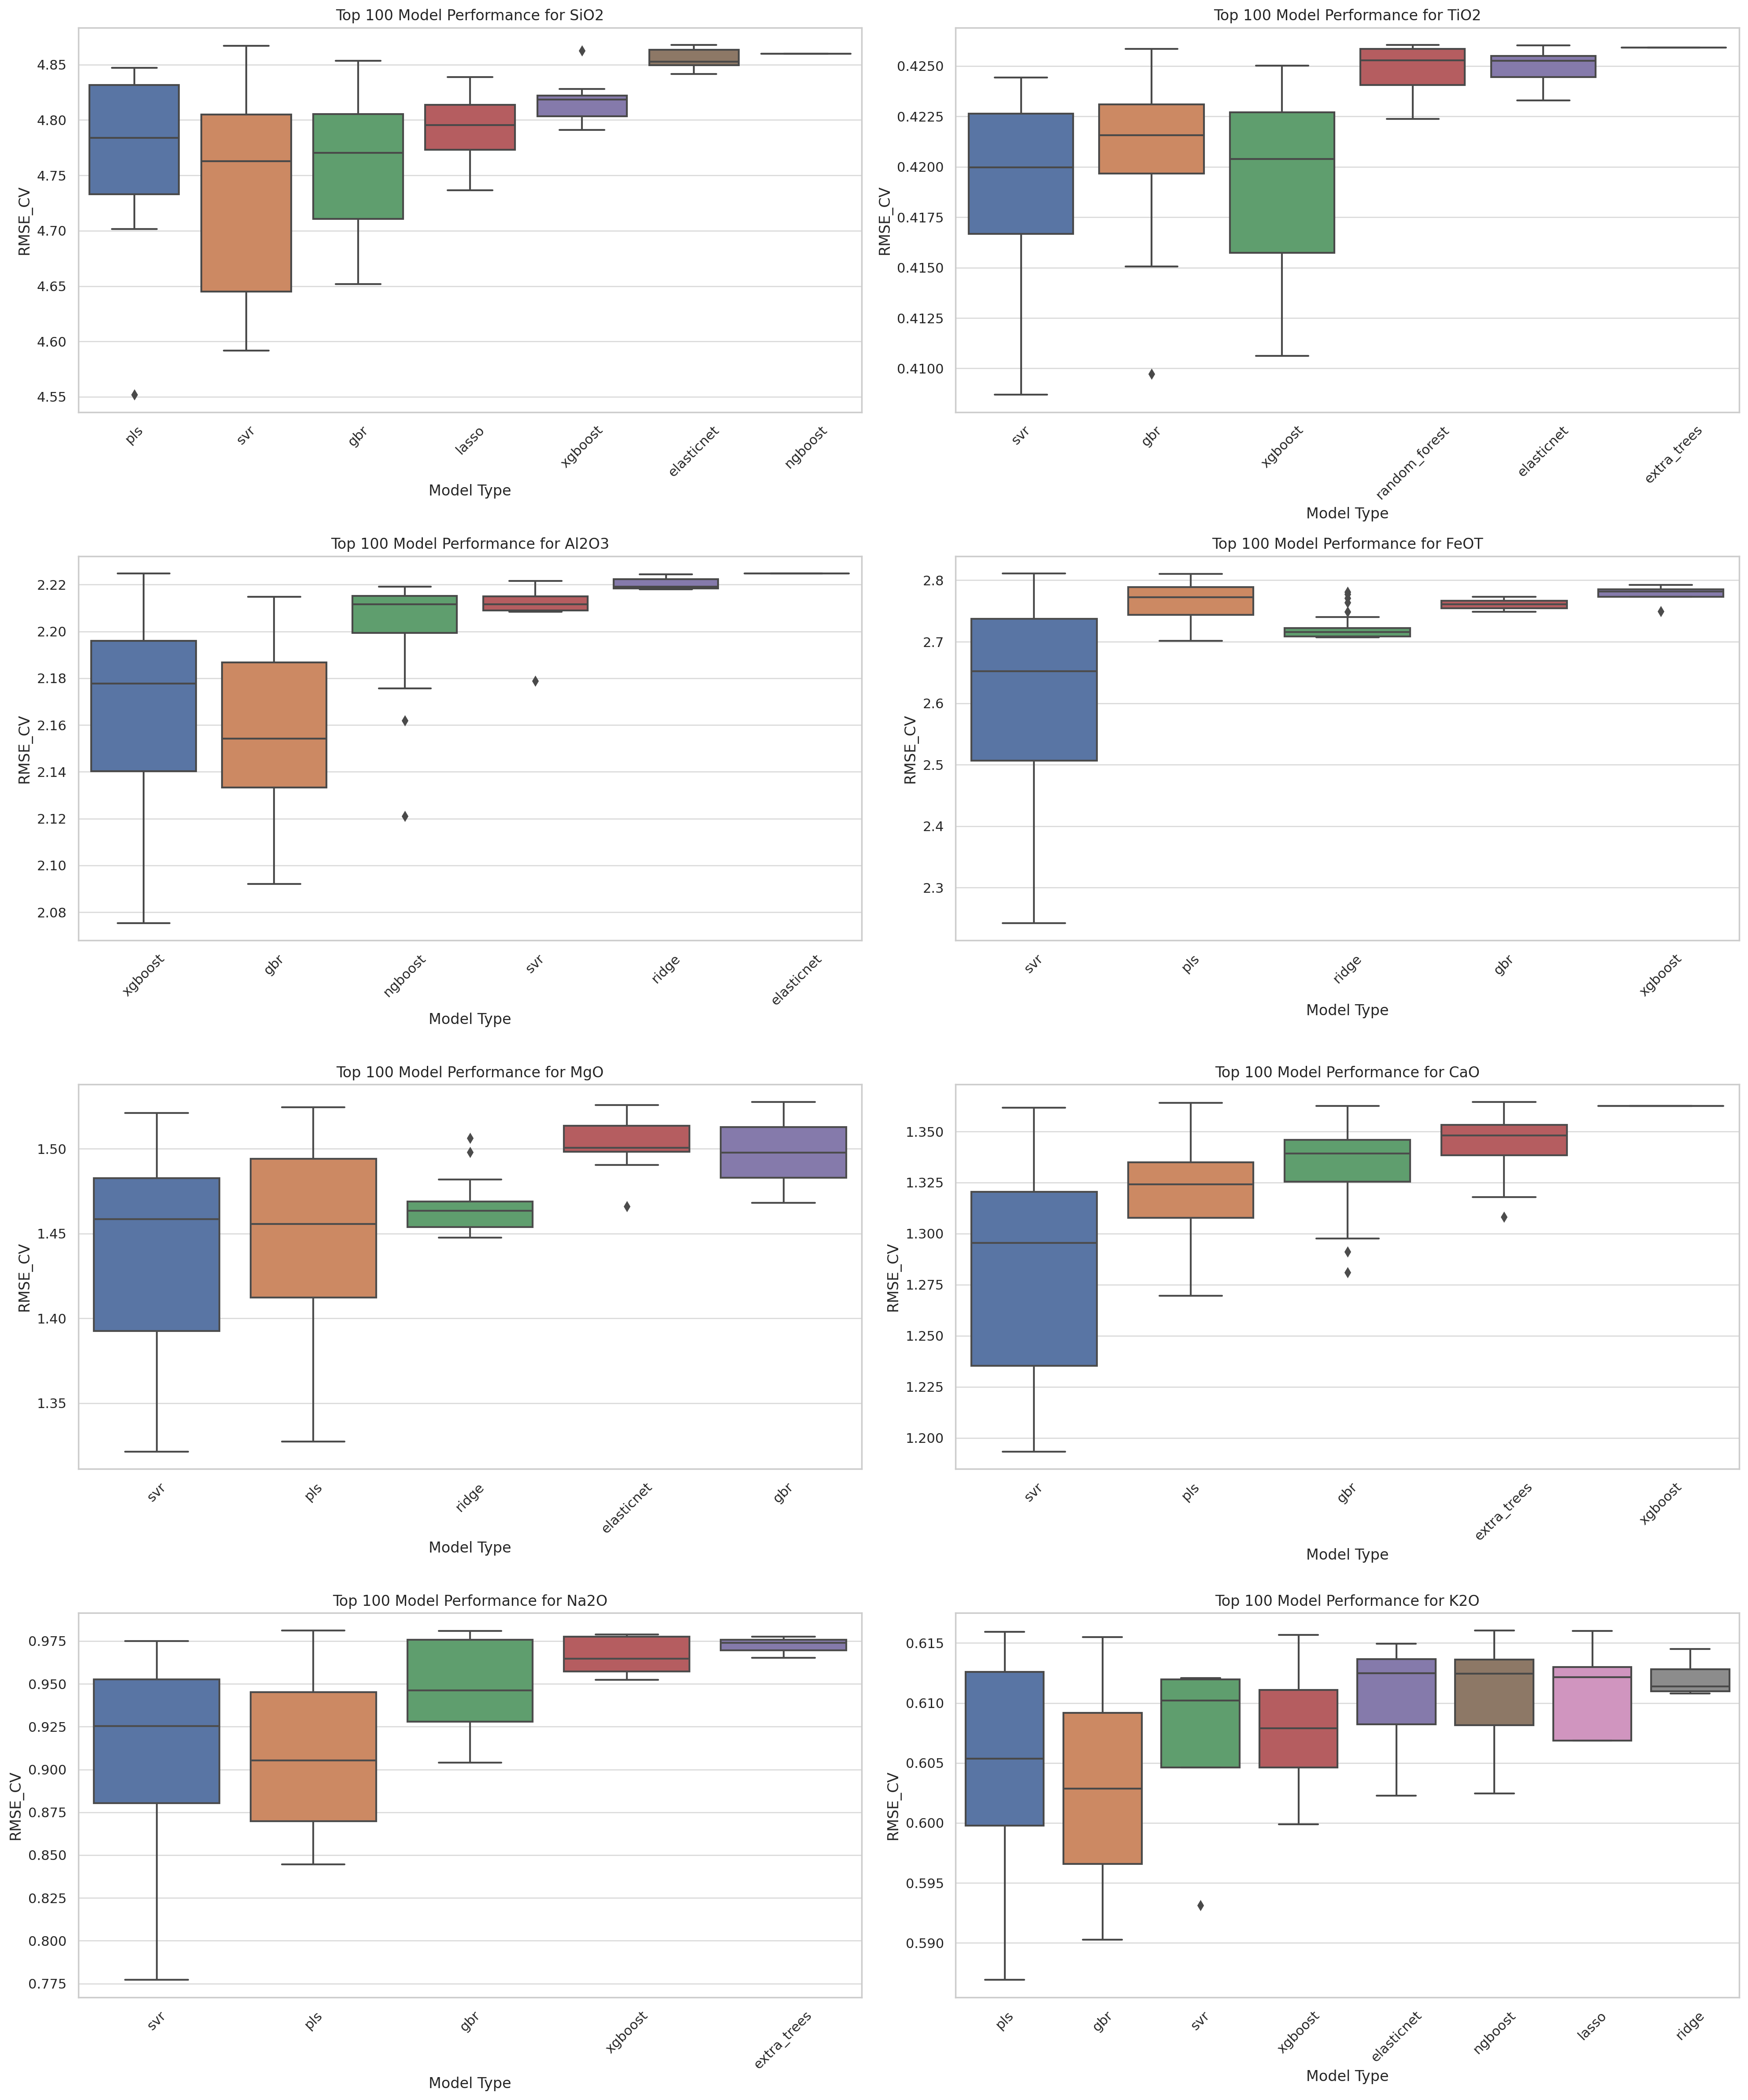
\includegraphics[width=\textwidth]{images/top100/models.png}
    \caption{Top 100 model performance across oxides. The subplots show the distribution of \gls{rmsecv} values for the top 100 trials for each model type across the eight different oxides. This helps identify the most effective models for each oxide within the top-performing trials.}
    \label{fig:top100_models}
\end{figure*}

\begin{figure*}
    \centering
    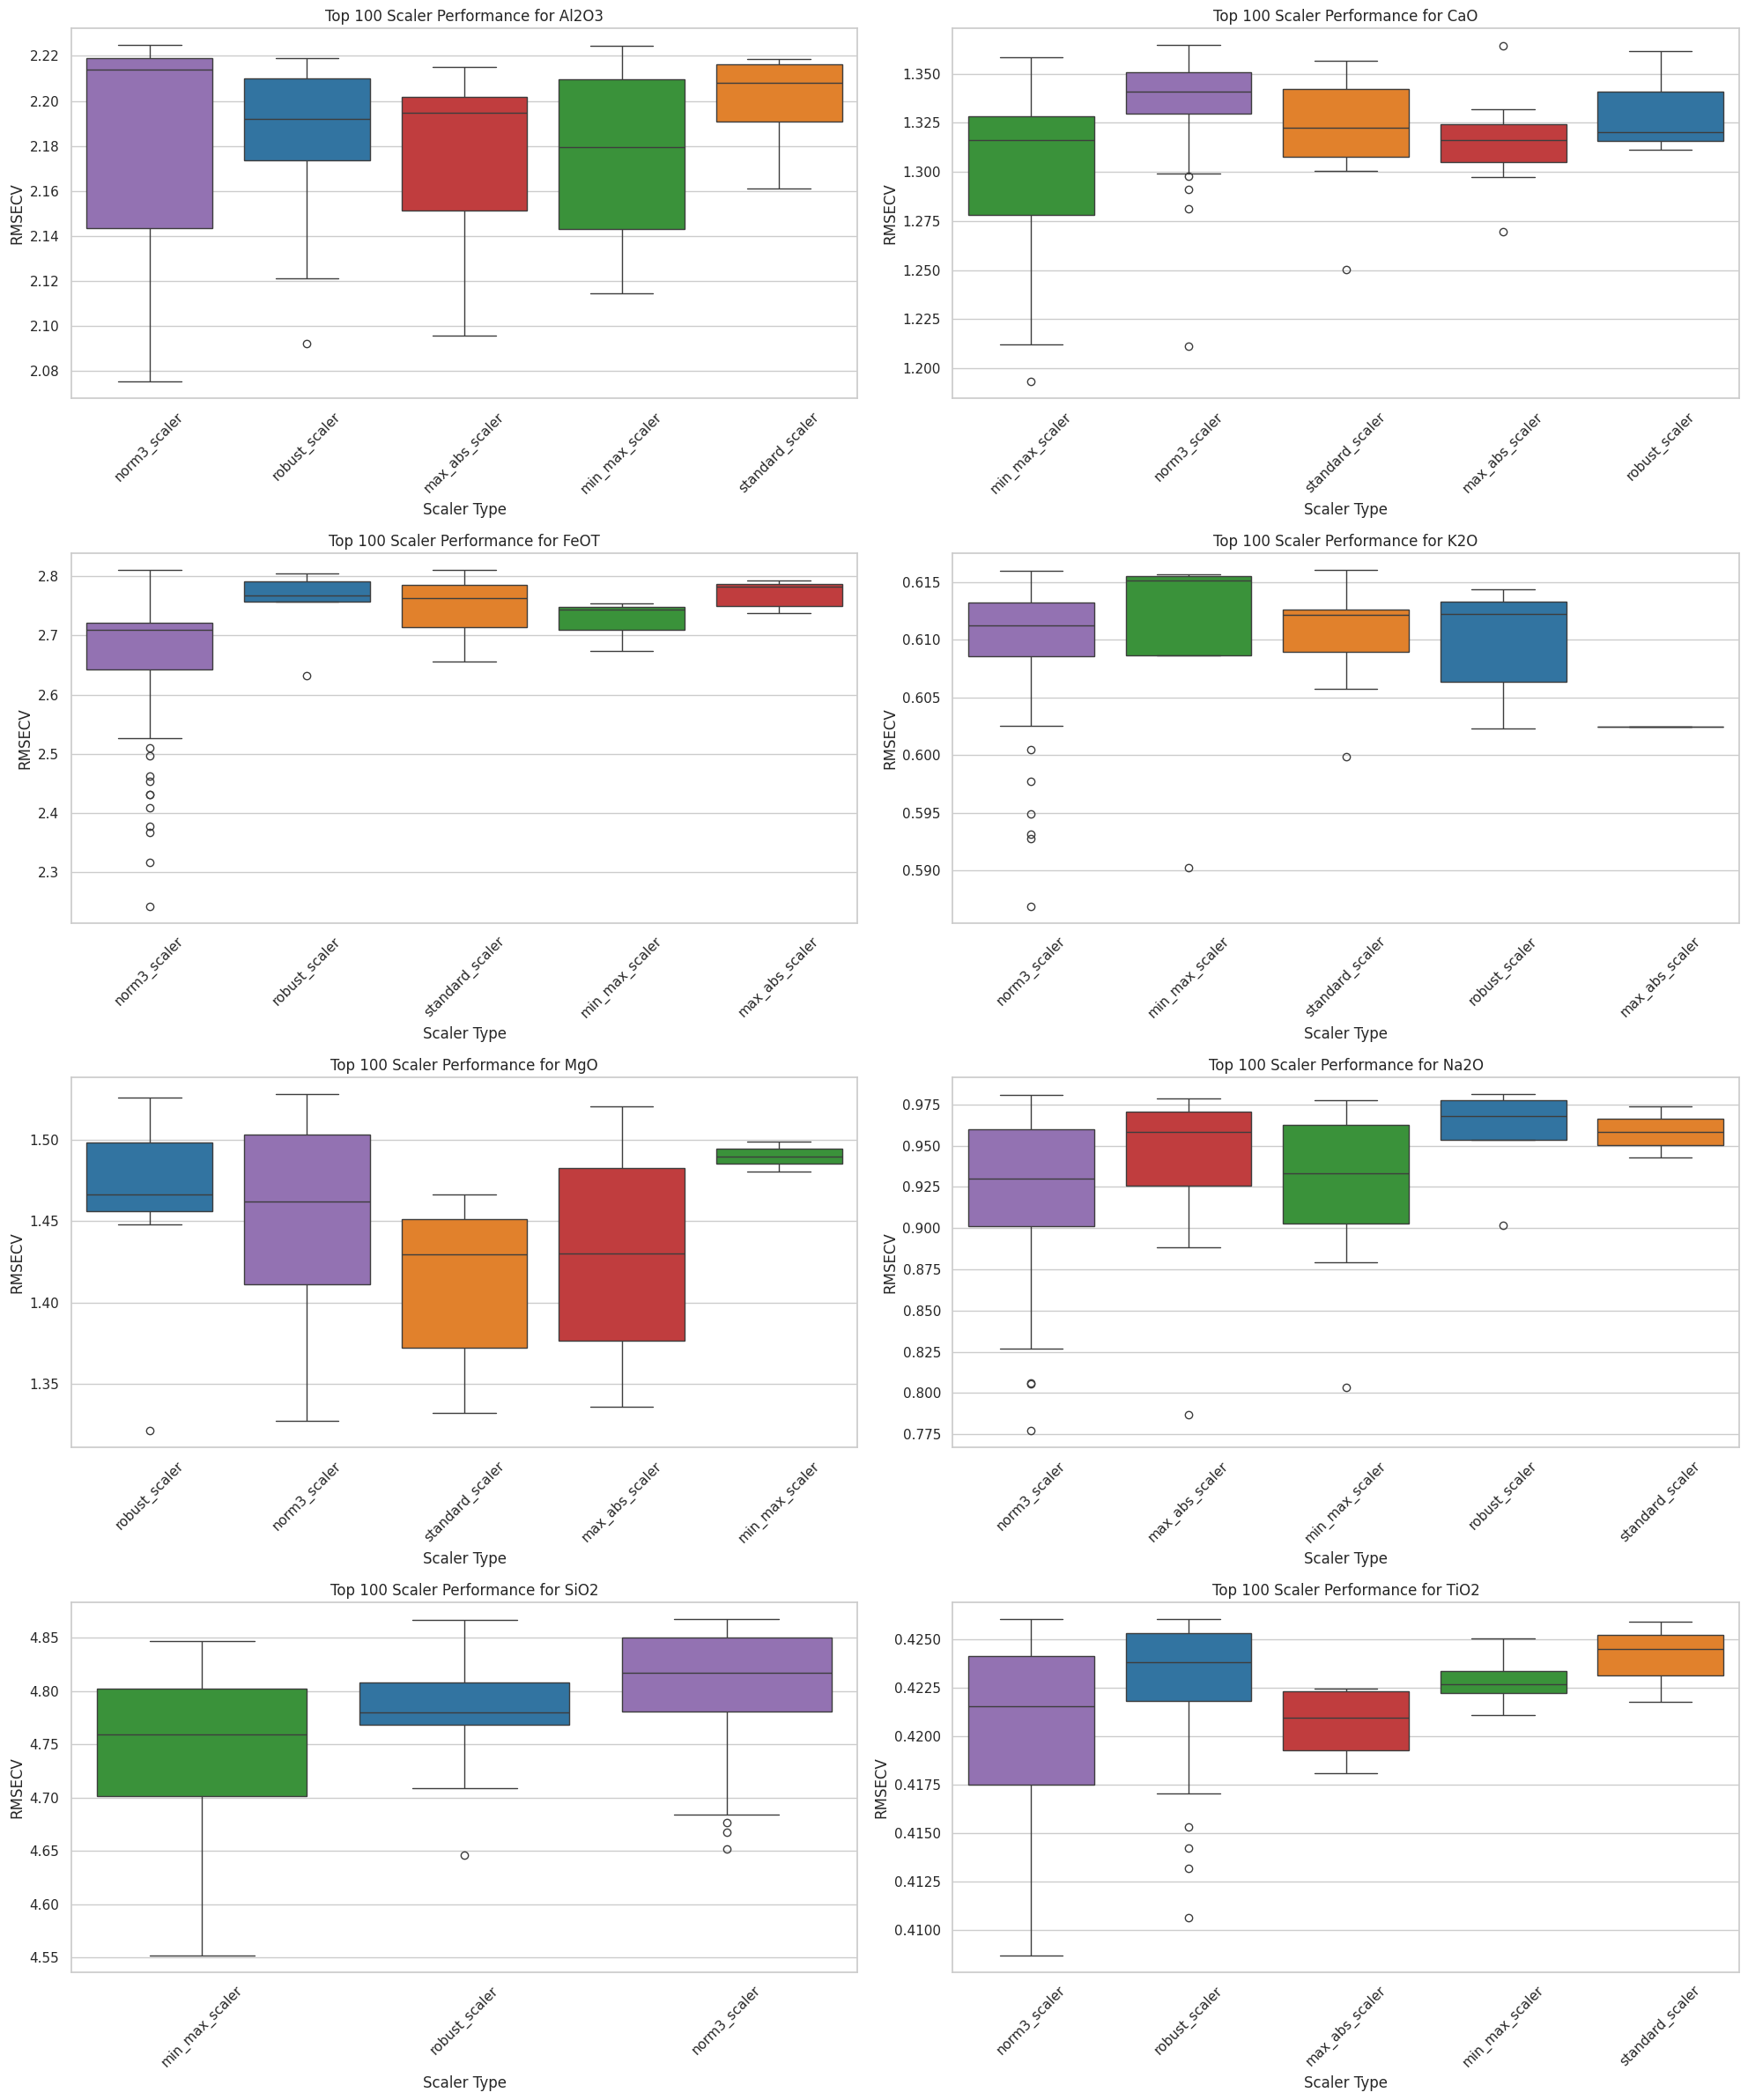
\includegraphics[width=\textwidth]{images/top100/scalers.png}
    \caption{Top 100 scaler performance across oxides. The subplots illustrate the distribution of \gls{rmsecv} values for the top 100 trials for each scaler type across the different oxides. This helps pinpoint which scalers perform best within the top-performing trials.}
    \label{fig:top100_scalers}
\end{figure*}

\begin{figure*}
    \centering
    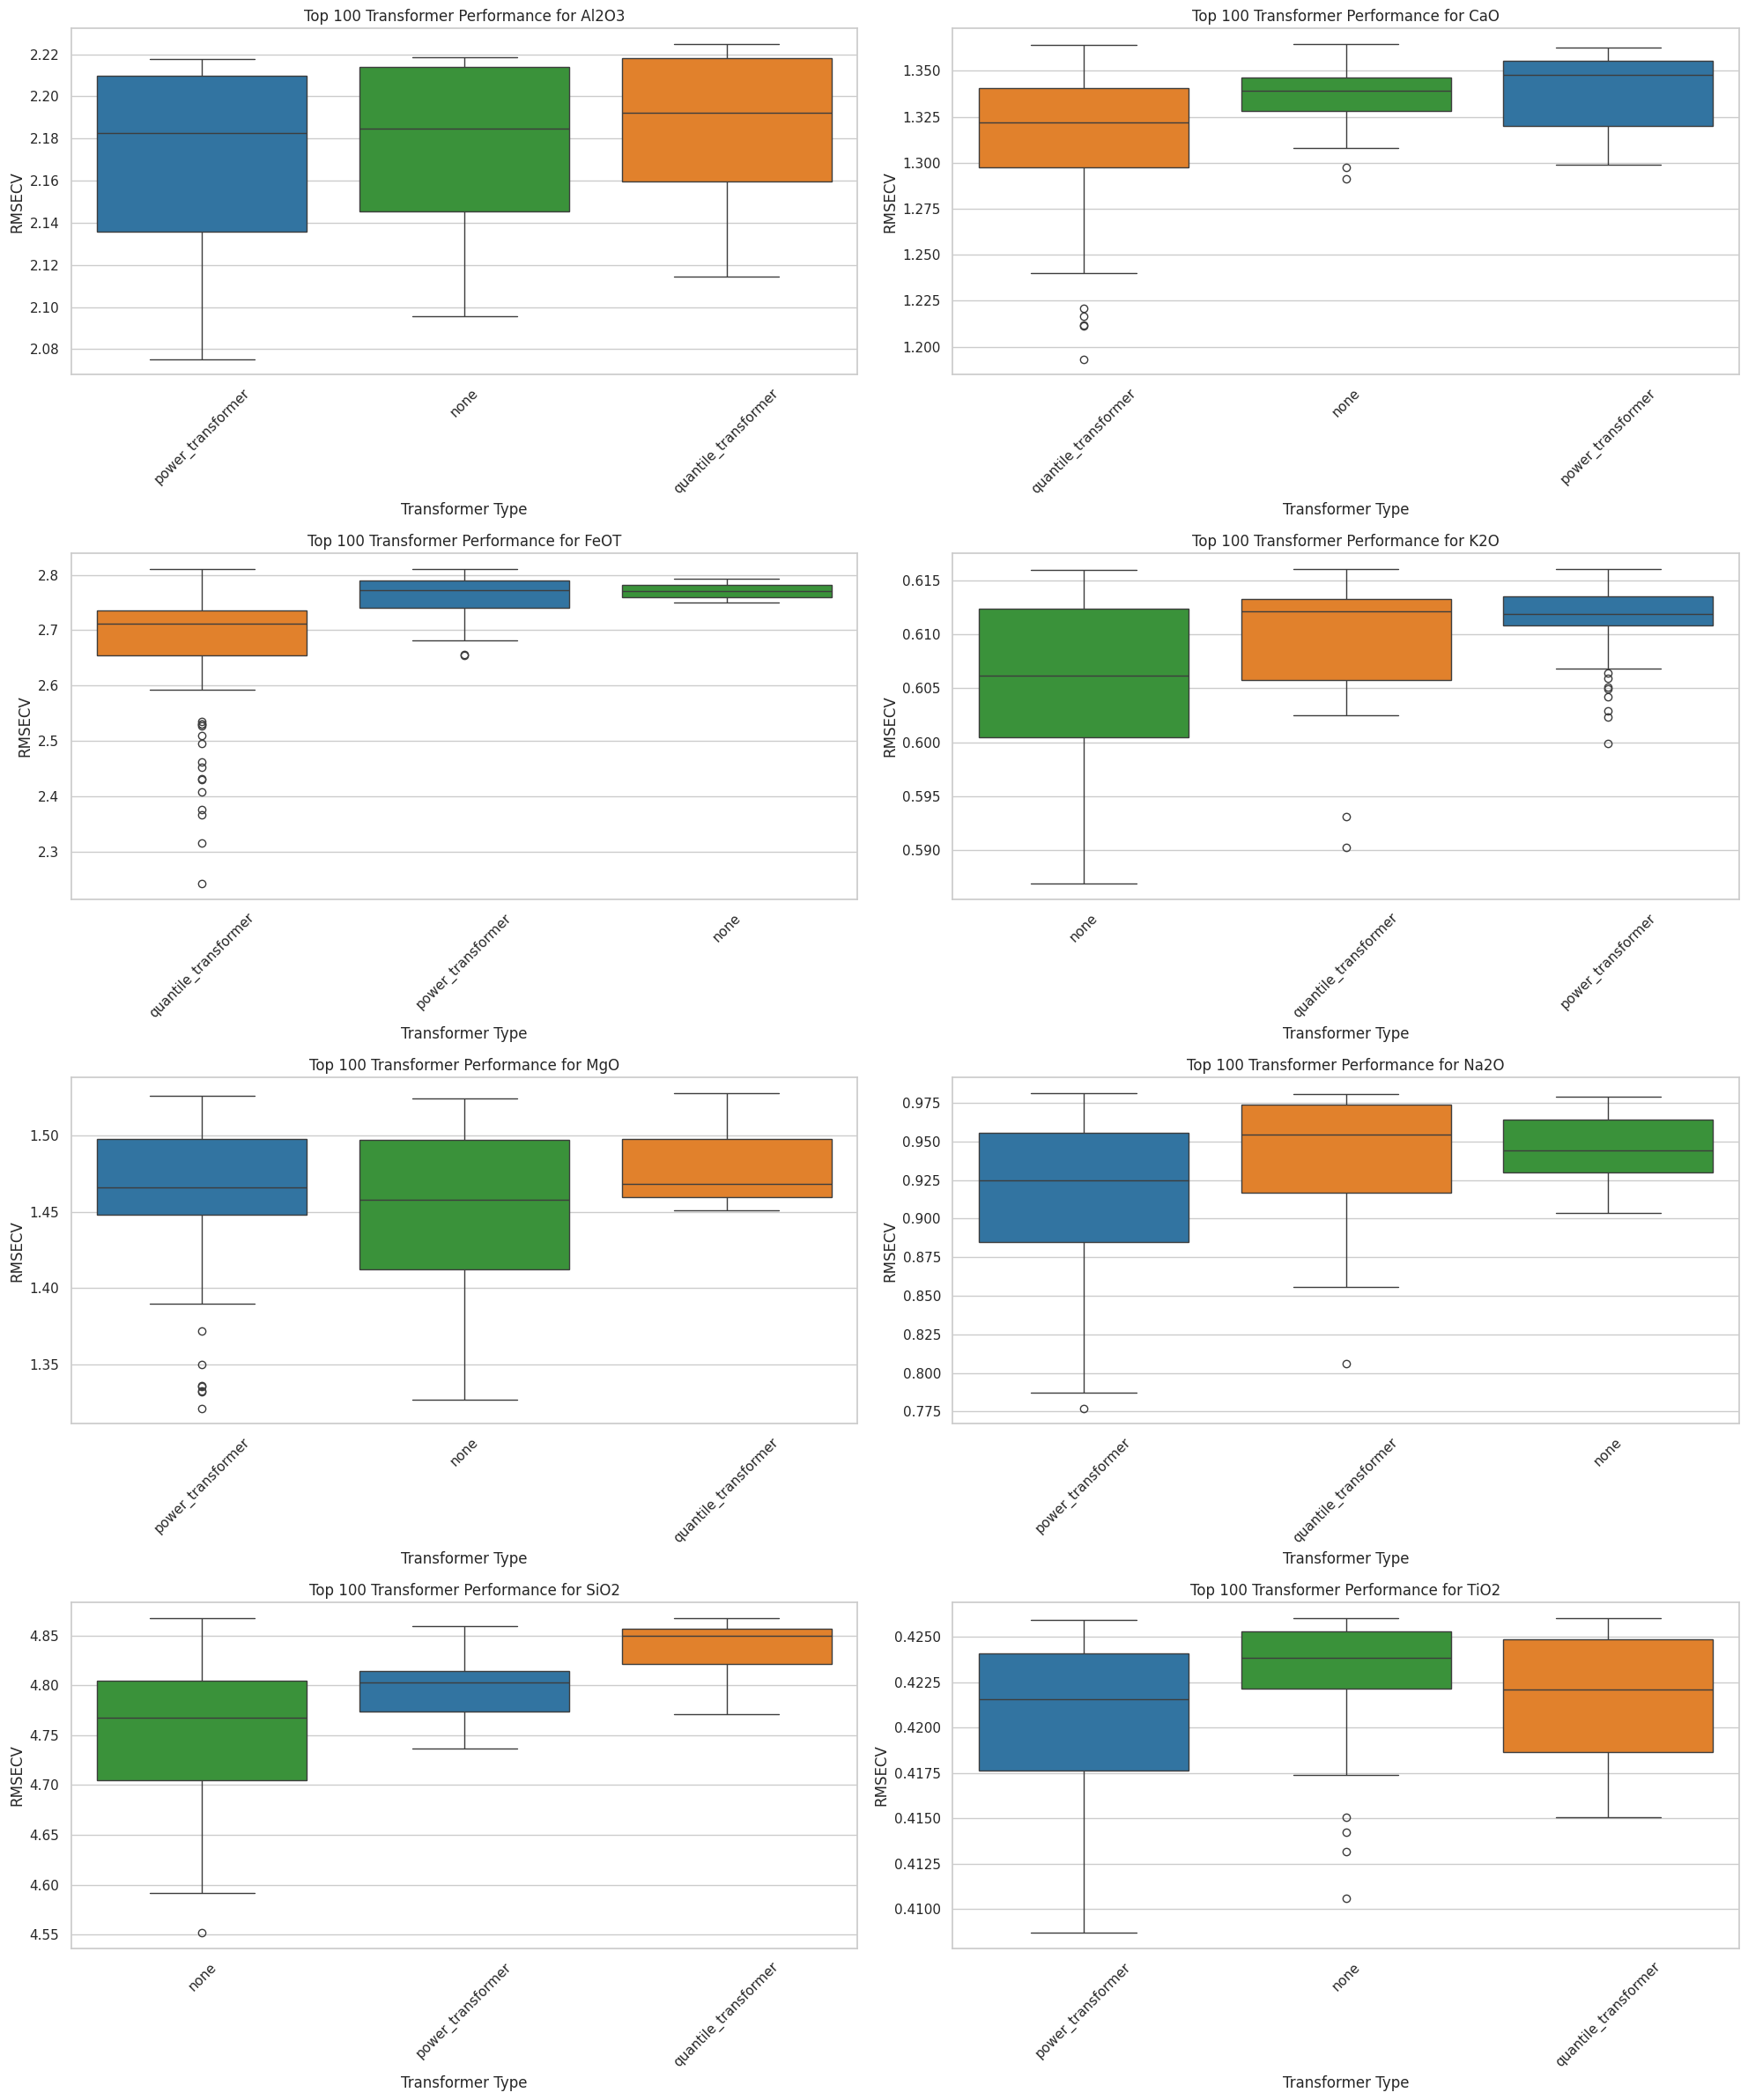
\includegraphics[width=\textwidth]{images/top100/transformers.png}
    \caption{Top 100 transformer performance across oxides. The subplots display the distribution of \gls{rmsecv} values for the top 100 trials for each transformer type across the different oxides. This helps determine the effectiveness of each transformer for different oxides within the top-performing trials.}
    \label{fig:top100_transformers}
\end{figure*}

\begin{figure*}
    \centering
    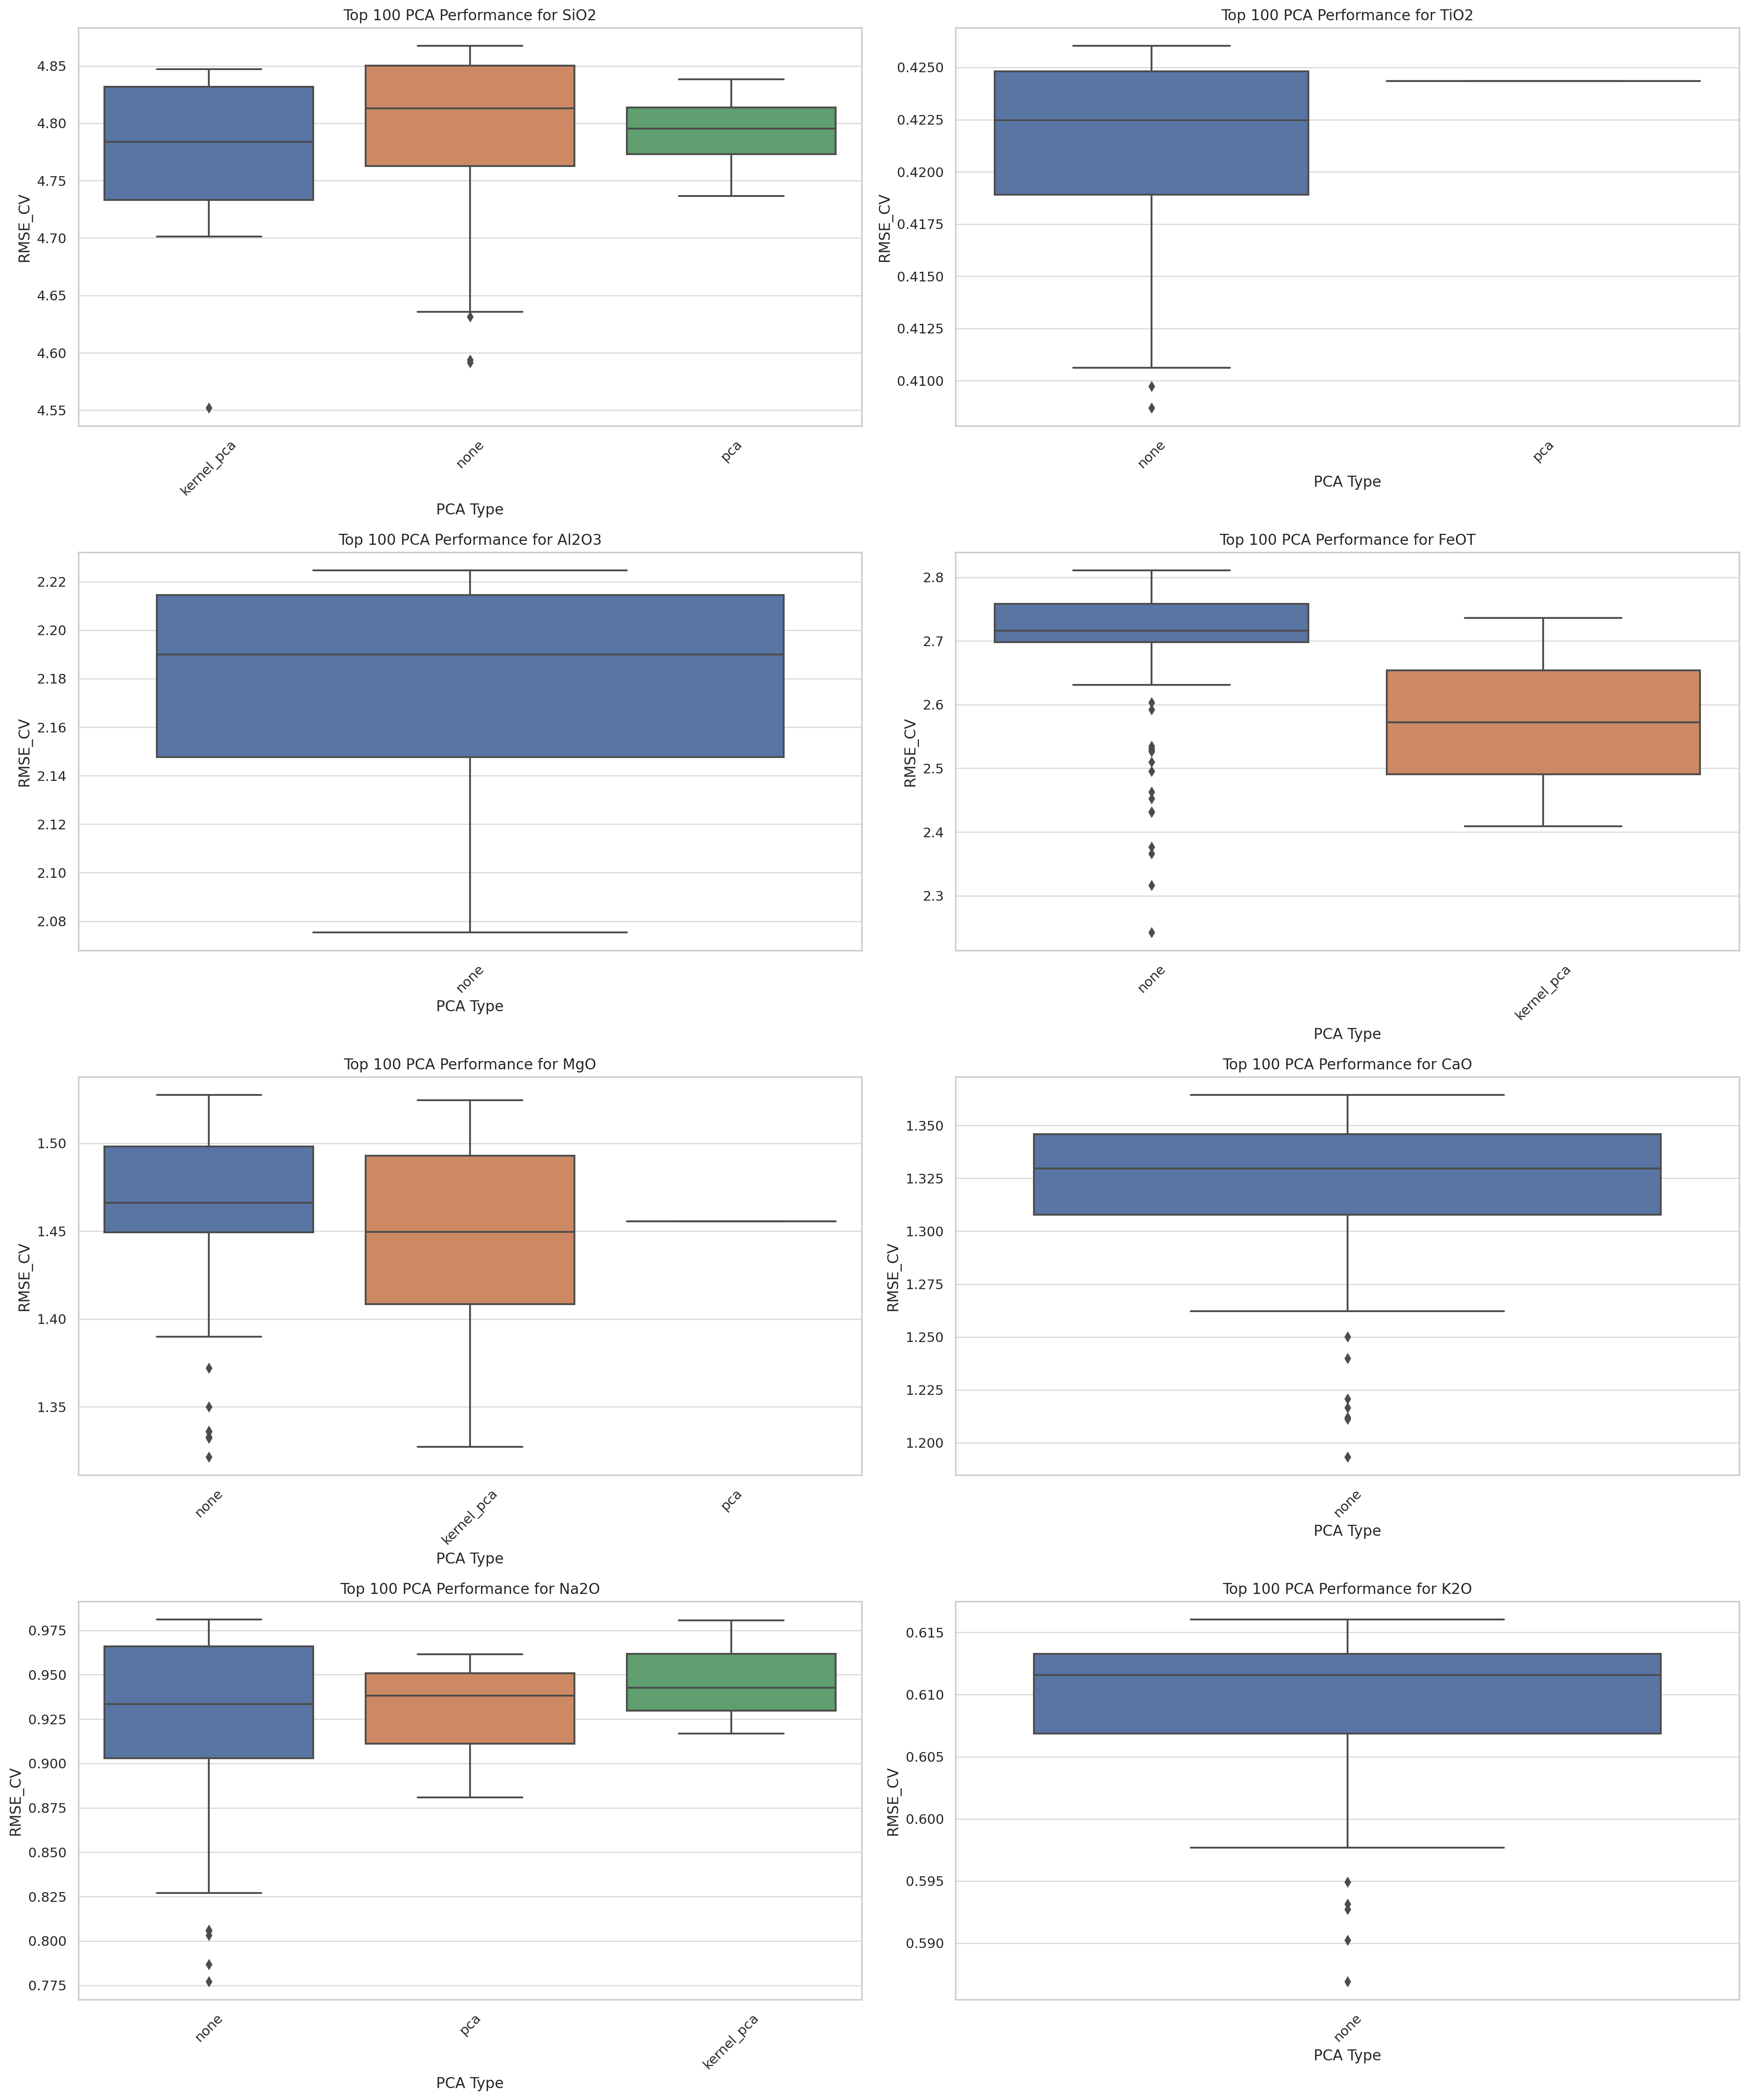
\includegraphics[width=\textwidth]{images/top100/pca.png}
    \caption{Top 100 \gls{pca} performance across oxides. The subplots present the distribution of \gls{rmsecv} values for the top 100 trials for each \gls{pca} type across the different oxides. This allows us to understand the impact of \gls{pca} techniques on model performance for each oxide within the top-performing trials.}
    \label{fig:top100_pca}
\end{figure*}

We conclude our analysis by presenting the best configurations for each oxide in Section~\ref{subsec:best_model_configurations}.
The section shows the single top-performing configurations for each model for each oxide, presented in Tables~\ref{tab:SiO2_best_configurations} through~\ref{tab:K2O_best_configurations}.
Similar to the previous plots, we use the \gls{rmsecv} values to determine the best configurations.
Notably, these tables illustrate how certain configurations may exhibit low \gls{rmsecv} values but relatively high \gls{rmsep} values.
This observation could suggest that they generalize well to the dataset containing extreme values but struggle with values closer to the mean.
For example, the top-performing configuration for \ce{SiO2} consists of \gls{pls} with \gls{kernel-pca} and \texttt{MinMaxScaler}.
This configuration has the lowest \gls{rmsecv} value of 4.55, but a relatively high \gls{rmsep} value of 4.08.
The next-best performing configuration for \ce{SiO2} is \gls{svr} with \texttt{MinMaxScaler}.
This configuration has a \gls{rmsecv} value of 4.59, but a \gls{rmsep} value of 3.53.
Although the difference in \gls{rmsecv} is negligible, the \gls{rmsep} value for the \gls{svr} configuration is much lower than that of the \gls{pls} configuration.
This indicates that the \gls{svr} configuration is likely a better overall predictor for \ce{SiO2} than the \gls{pls} configuration.

The analysis of the best configurations for each oxide reveals that certain models and preprocessing techniques consistently outperform others. \gls{svr} and \gls{pls} models, in particular, frequently appear among the top configurations. The use of transformers such as the Power Transformer and scalers like Norm 3 and Min-Max Scaler are also common among the best configurations.

Finally, we use a combination of these top-performing configurations by selecting the top-$n$ performing configurations per oxide for our stacking ensemble.
This approach is further elaborated on in Section~\ref{subsec:stacking_ensemble}.
\subsection{Stacking Ensemble}\label{subsec:stacking_ensemble}
Given the results of the optimization process, we implemented a stacking ensemble to combine the predictions of the top-performing configurations.
As with all our experiments, we follow the procedure outlined in Section~\ref{subsec:validation_testing_procedures} to evaluate the performance of the stacking ensemble.

For each oxide, we first identified the top-performing configurations to use in the stacking ensemble.
To identify the top-performing configurations for use in the stacking ensemble, we developed a category-based method that groups models into distinct categories for systematic comparison.
This approach helps in selecting models that perform optimally for specific tasks while ensuring diversity within the ensemble.
Additionally, we developed and employed a grid search to identify the optimal ensemble configurations, but time constraints prevented us from fully completing this process.
Finally, we employed the stacking model and evaluated its performance.
We present the results as well as the 1:1 plots in Section~\ref{subsec:stacking_ensemble_results}.

\subsubsection{Category Method \& Pipeline Selection}\label{subsec:category_method}
The category-based method organizes models into the following groups:

\begin{itemize}
    \item Gradient Boosting: \gls{gbr}, \gls{xgboost}, \gls{ngboost}
    \item Tree-Based: \gls{etr}, \gls{rf}
    \item Linear and Regularized Models: \gls{lasso}, Ridge, \gls{enet}
    \item SVM: \gls{svr}
    \item PLS: \gls{pls}
\end{itemize}

We used the top-performing configurations identified in Section~\ref{sec:optimization_results} to select configurations for the stacking ensemble.

For each oxide, we filtered the trial data from the optimization experiment to create a dataset containing configuration information and performance metrics.
These datasets were sorted by \gls{rmsecv}.
We then selected unique model types for further analysis, based on the categories above.
Our process involved selecting a set number of configurations for each category until a maximum number of configurations for the oxide's ensemble was reached.

To ensure diversity and limit scope, we set a maximum of one model per category and three models per stacking ensemble, with one ensemble for each oxide.
For each oxide, we developed pipelines to preprocess the data according to the given configuration and to utilize the models with their optimal hyperparameters.
These pipelines represent the optimal configurations for each oxide, and are used as base estimators in the stacking ensemble.

\subsubsection{Grid Search}\label{subsec:grid_search}
The grid search process begins by generating all possible combinations of the selected models.
Specifically, we generate combinations with at least two models, up to a configurable maximum number of models.

For each oxide, we constructed a pipeline for each of the top model configurations identified in Section~\ref{sec:optimization_results}.
The evaluation function iterates over each combination of base estimators, constructs a stacking ensemble pipeline, and assesses its performance using cross-validation.

The evaluation function prepares the pipeline with the current combination of base estimators and splits the data into training and testing sets using our data partitioning method.
The stacking ensemble is then fitted on the training set, and the meta-features generated from the base estimators are used to train the final estimator.

We compute the evaluation metrics to assess the ensemble's effectiveness.
The best combination is identified based on the lowest \gls{rmsecv} value.

It is possible to vary the meta-learner in this process, adding another variable to tune as part of the search process.

While our grid search implementation was limited to the \ce{TiO2} oxide, the methodology demonstrates the potential for identifying optimal stacking ensembles by systematically evaluating model combinations and their configurations.
We chose not to pursue this method further due to the time constraints of this project, but believe it is a promising approach for future work.


\subsubsection{Results}\label{subsec:stacking_ensemble_results}
For each major oxide, we ran the stacking ensemble and evaluated its performance.
The evaluations were conducted using the same configurations, varying only the meta-learner between runs.
We present the results for the \gls{enet} meta-learner with \texttt{alpha} = 1.0, as well as for the \gls{enet} meta-learner with \texttt{alpha} = 0.1.
Additionally, we present the results for the \gls{svr} meta-learner, using the default hyperparameters provided by \texttt{scikit-learn}.

The evaluation metrics are shown in Table~\ref{tab:stacking_ensemble_results_enet}, Table~\ref{tab:stacking_ensemble_results_enet_01}, and Table~\ref{tab:stacking_ensemble_results_svr}.
Additionally, we provide 1:1 plots for each ensemble in Figures~\ref{fig:elasticnet_one_to_one}, \ref{fig:enetalpha01_one_to_one}, and \ref{fig:svr_one_to_one}, showing the actual versus predicted values for each oxide.

A notable observation from our results is that different meta-learners exhibited varying performance levels across oxides.
We observed that the final predictions were strongly affected by the meta-learner, going as far as rendering some predictions nonsensical if the wrong meta-learner was chosen.
Specifically, for \ce{TiO2}, we observed that predictions remained near-constant values despite varying the combination of model configurations in the \ce{TiO2} ensemble.
In fact, this was the reason for our implementation of the grid search process.
The consistency of our observations supported our hypothesis: changing only the meta-learner significantly impacts the \gls{rmsecv} and prediction outcomes.
We decided to investigate further and identified potential issues with small value predictions when using an \gls{enet} meta-learner.
For example, most values for \ce{TiO2} fell between 0 and 2.5, as shown in Figure~\ref{fig:oxide_distributions}.
The regularization term likely dominated the fitting process, leading to underfitting and resulting in nearly constant predictions.
This hypothesis was confirmed by adjusting the regularization parameter, \texttt{alpha}, in the \gls{enet}.
Lowering \texttt{alpha} produced better outcomes, indicating that regularization adversely affected the predicted values.
The 1:1 plot in Figure~\ref{fig:elasticnet_one_to_one} shows the near-constant predictions for \ce{TiO2} when using a \gls{enet} meta-learner, and Figure~\ref{fig:enetalpha01_one_to_one} shows the improved predictions with \texttt{alpha} = 0.1.
This leads us to conclude that the meta-learner's choice significantly impacts the \gls{rmsecv} and prediction outcomes.

The stacking approach demonstrated strong improvements in prediction accuracy compared to the baseline described in Section~\ref{sec:baseline_replica}, validating the efficacy of our methodology.
We measured this improvement using \gls{rmsep}, which provides the fairest comparison between the baseline and the stacking approach.
As mentioned, \gls{rmsep} evaluates the model's performance on the test set.
In Section~\ref{sec:baseline_replica}, we described how the baseline test set was constructed by sorting extreme concentration values into the training set, and then performing a random split.
As noted in Section~\ref{subsec:validation_testing_procedures}, a more sophisticated procedure is required to support the testing and validation strategy in this work.
Despite the differences in test set construction, the test sets remained similar in composition\footnote{The analysis of this can be found on our GitHub repository: \url{https://github.com/chhoumann/thesis-chemcam}}, which allowed us to use \gls{rmsep} as a fair comparison metric.
Table~\ref{tab:stacking_ensemble_vs_moc} compares the \gls{rmsep} values of different oxides for the \gls{moc} (replica) model with three stacking ensemble models: \gls{enet} with $\alpha = 1$, \gls{enet} with $\alpha = 0.1$, and \gls{svr}.
Overall, the stacking ensemble models tend to produce lower \gls{rmsep} values compared to the \gls{moc} (replica) model.
Notably, \ce{SiO2}, \ce{TiO2}, \ce{Na2O}, and \ce{K2O} show large improvements across all stacking ensemble models.
For instance, the \gls{rmsep} for \ce{SiO2} is reduced from 5.61 (\gls{moc} (replica)) to around 3.59 (\gls{enet} with $\alpha = 1$) and further to 3.47 (\gls{svr}).
Similarly, \ce{TiO2} shows a reduction from 0.61 (\gls{moc} (replica)) to 0.32 (\gls{enet} with $\alpha = 0.1$).
The improvements are consistent across most oxides, with \gls{enet} and \gls{svr} models both outperforming the \gls{moc} (replica) model.
This shows that the ensemble approach, particularly with these meta-learners, enhances prediction accuracy for the oxides we tested.

The results presented above indicate a strong performance from the stacking ensemble approach.
However, it is important to note that some evaluation metrics are worse in the stacking approach than in certain individual configurations.
We believe that further tuning, particularly of the meta-learner's hyperparameters, could substantially improve these results.

\begin{table}
\centering
\caption{Stacking ensemble results using the \gls{enet} model as the meta-learner with $\alpha = 1$.}
\begin{tabular}{lcccc}
\toprule
Oxide          & \gls{rmsep} & STDDEV & \gls{rmsecv}         & Std. Dev. CV          \\
\midrule
\ce{SiO2}      & 3.588       & 3.582  & 4.680 $\pm$ 0.500    & 4.670 $\pm$ 0.516     \\
\ce{TiO2}      & 0.571       & 0.565  & 0.818 $\pm$ 0.111    & 0.814 $\pm$ 0.117     \\
\ce{Al2O3}     & 1.656       & 1.657  & 2.211 $\pm$ 0.023    & 2.199 $\pm$ 0.226     \\
\ce{FeO_T}     & 1.794       & 1.789  & 2.792 $\pm$ 0.649    & 2.745 $\pm$ 0.646     \\
\ce{MgO}       & 0.711       & 0.711  & 1.660 $\pm$ 0.525    & 1.635 $\pm$ 0.516     \\
\ce{CaO}       & 1.636       & 1.619  & 1.307 $\pm$ 0.205    & 1.290 $\pm$ 0.202     \\
\ce{Na2O}      & 0.470       & 0.462  & 1.075 $\pm$ 0.706    & 1.067 $\pm$ 0.710     \\
\ce{K2O}       & 0.476       & 0.462  & 0.653 $\pm$ 0.195    & 0.652 $\pm$ 0.193     \\
\bottomrule
\end{tabular}
\label{tab:stacking_ensemble_results_enet}
\end{table}

\begin{table}
\centering
\caption{Stacking ensemble results using the \gls{enet} model as the meta-learner with $\alpha = 0.1$.}
\begin{tabular}{lcccc}
\toprule
Oxide          & \gls{rmsep} & STDDEV & \gls{rmsecv}         & Std. Dev. CV          \\
\midrule
\ce{SiO2}      & 3.598       & 3.591  & 4.686 $\pm$ 0.489    & 4.677 $\pm$ 0.505     \\
\ce{TiO2}      & 0.319       & 0.310  & 0.450 $\pm$ 0.083    & 0.448 $\pm$ 0.083     \\
\ce{Al2O3}     & 1.658       & 1.660  & 2.192 $\pm$ 0.235    & 2.180 $\pm$ 0.238     \\
\ce{FeO_T}     & 1.841       & 1.840  & 2.781 $\pm$ 0.664    & 2.731 $\pm$ 0.659     \\
\ce{MgO}       & 0.768       & 0.768  & 1.632 $\pm$ 0.531    & 1.608 $\pm$ 0.518     \\
\ce{CaO}       & 1.647       & 1.627  & 1.310 $\pm$ 0.213    & 1.291 $\pm$ 0.211     \\
\ce{Na2O}      & 0.442       & 0.433  & 1.093 $\pm$ 0.690    & 1.079 $\pm$ 0.692     \\
\ce{K2O}       & 0.494       & 0.477  & 0.556 $\pm$ 0.155    & 0.553 $\pm$ 0.153     \\
\bottomrule
\end{tabular}
\label{tab:stacking_ensemble_results_enet_01}
\end{table}

\begin{table}
\centering
\caption{Stacking ensemble results using the \gls{svr} model as the meta-learner with default hyperparameters.}
\begin{tabular}{lcccc}
\toprule
Oxide          & \gls{rmsep} & STDDEV & \gls{rmsecv}         & Std. Dev. CV          \\
\midrule
\ce{SiO2}      & 3.473       & 3.478  & 5.064 $\pm$ 0.932    & 5.061 $\pm$ 0.926     \\
\ce{TiO2}      & 0.340       & 0.333  & 0.442 $\pm$ 0.087    & 0.442 $\pm$ 0.087     \\
\ce{Al2O3}     & 1.729       & 1.732  & 2.285 $\pm$ 0.226    & 2.274 $\pm$ 0.233     \\
\ce{FeO_T}     & 1.693       & 1.681  & 4.821 $\pm$ 1.490    & 4.768 $\pm$ 1.495     \\
\ce{MgO}       & 0.819       & 0.820  & 2.569 $\pm$ 1.274    & 2.559 $\pm$ 1.271     \\
\ce{CaO}       & 1.594       & 1.574  & 1.475 $\pm$ 0.294    & 1.456 $\pm$ 0.304     \\
\ce{Na2O}      & 0.369       & 0.368  & 0.978 $\pm$ 0.885    & 0.971 $\pm$ 0.887     \\
\ce{K2O}       & 0.511       & 0.497  & 0.669 $\pm$ 0.199    & 0.666 $\pm$ 0.196     \\
\bottomrule
\end{tabular}
\label{tab:stacking_ensemble_results_svr}
\end{table}

\begin{figure*}
    \centering
    \resizebox{0.75\textwidth}{!}{
        \begin{tabular}{cc}
            \begin{subfigure}{0.5\textwidth}
                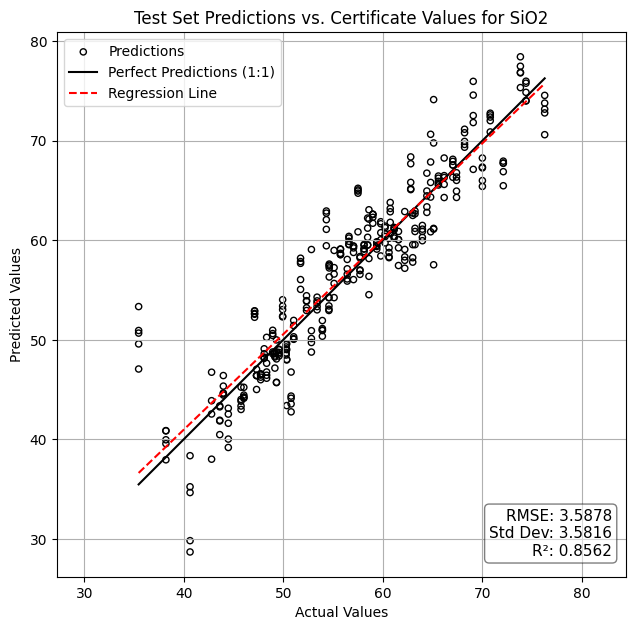
\includegraphics[width=\textwidth]{images/one_to_one/elasticnet/SiO2.png}
            \end{subfigure} & \hspace{3cm}
            \begin{subfigure}{0.5\textwidth}
                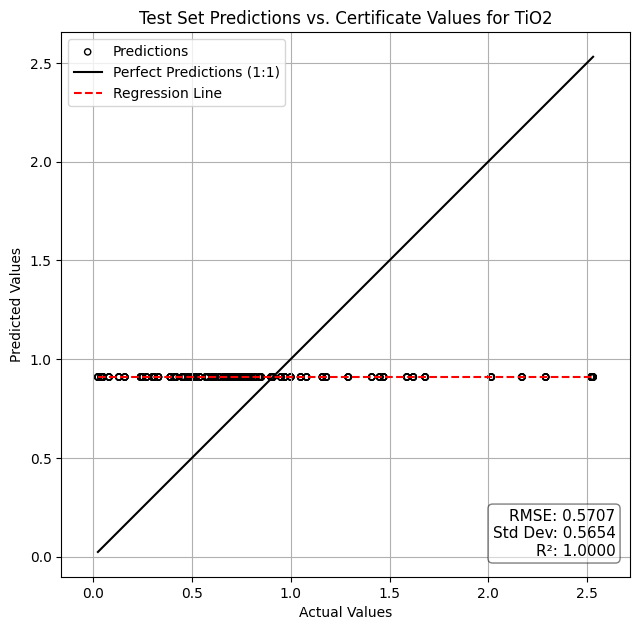
\includegraphics[width=\textwidth]{images/one_to_one/elasticnet/TiO2.png}
            \end{subfigure} \\
            \begin{subfigure}{0.5\textwidth}
                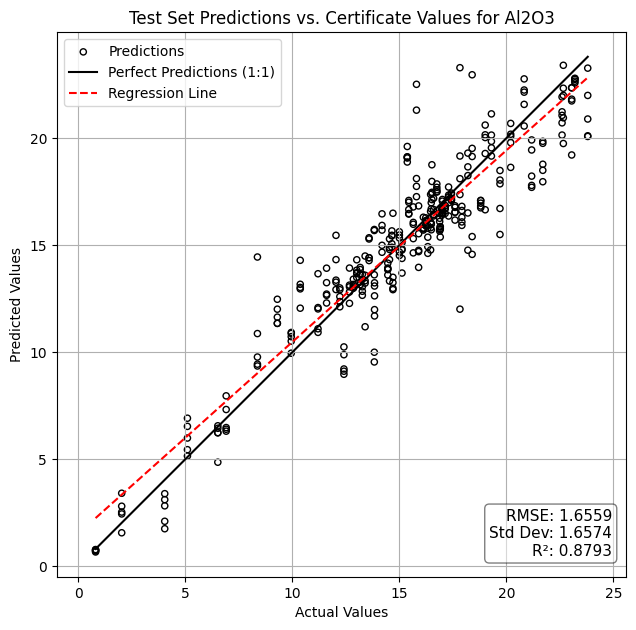
\includegraphics[width=\textwidth]{images/one_to_one/elasticnet/Al2O3.png}
            \end{subfigure} & \hspace{3cm}
            \begin{subfigure}{0.5\textwidth}
                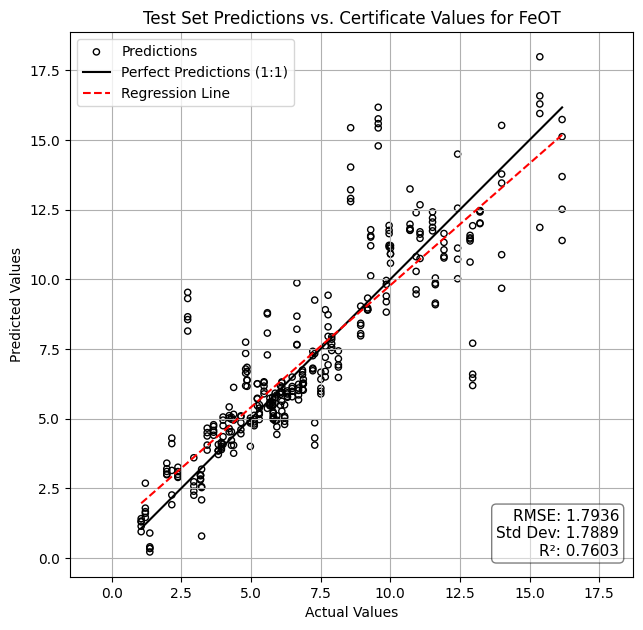
\includegraphics[width=\textwidth]{images/one_to_one/elasticnet/FeOT.png}
            \end{subfigure} \\
            \begin{subfigure}{0.5\textwidth}
                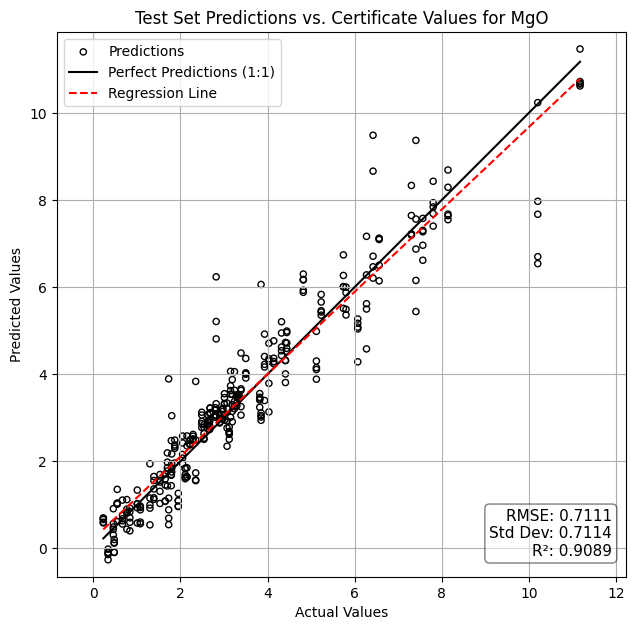
\includegraphics[width=\textwidth]{images/one_to_one/elasticnet/MgO.png}
            \end{subfigure} & \hspace{3cm}
            \begin{subfigure}{0.5\textwidth}
                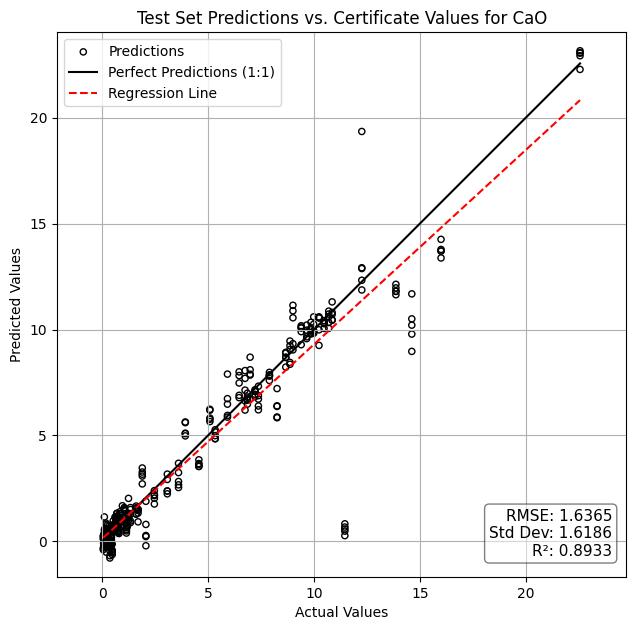
\includegraphics[width=\textwidth]{images/one_to_one/elasticnet/CaO.png}
            \end{subfigure} \\
            \begin{subfigure}{0.5\textwidth}
                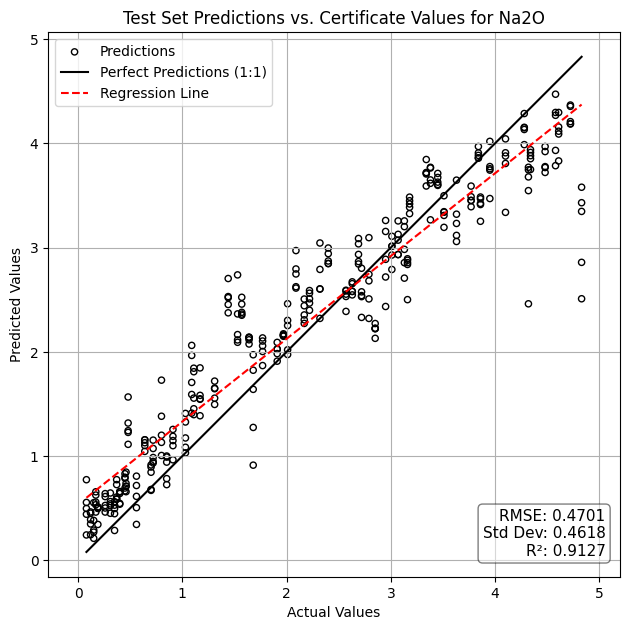
\includegraphics[width=\textwidth]{images/one_to_one/elasticnet/Na2O.png}
            \end{subfigure} & \hspace{3cm}
            \begin{subfigure}{0.5\textwidth}
                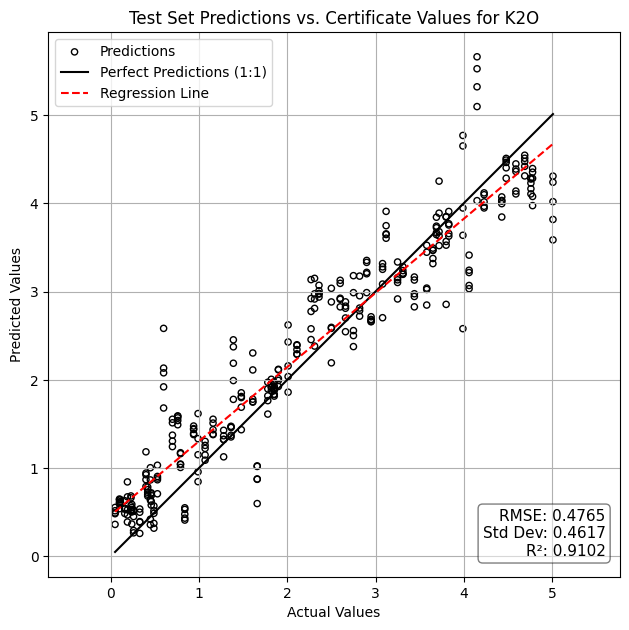
\includegraphics[width=\textwidth]{images/one_to_one/elasticnet/K2O.png}
            \end{subfigure}
        \end{tabular}
    }
    \caption{One-to-one plots for the stacking ensemble model with the \gls{enet} as the meta-learner with $\alpha = 1$}
    \label{fig:elasticnet_one_to_one}
\end{figure*}

\begin{table}
\centering
\caption{Comparison of \gls{rmsep} values for the \gls{moc} (replica) model and various stacking ensemble models.}
\resizebox{0.45\textwidth}{!}{
\begin{tabular}{lccccc}
\toprule
Oxide          & \gls{moc} (replica) & \gls{enet} ($\alpha = 1$) & \gls{enet} ($\alpha = 0.1$) & \gls{svr} \\
\midrule
\ce{SiO2}      & 5.61          & 3.59              & 3.60                & \textbf{3.47} \\
\ce{TiO2}      & 0.61          & 0.57              & \textbf{0.32}       & 0.34 \\
\ce{Al2O3}     & 2.47          & \textbf{1.66}     & 1.66                & 1.73 \\
\ce{FeO_T}     & 1.82          & 1.79              & 1.84                & \textbf{1.69} \\
\ce{MgO}       & 1.56          & \textbf{0.71}     & 0.77                & 0.82 \\
\ce{CaO}       & 2.09          & \textbf{1.64}     & 1.65                & 1.59 \\
\ce{Na2O}      & 1.33          & 0.47              & 0.44                & \textbf{0.37} \\
\ce{K2O}       & 1.91          & \textbf{0.48}     & 0.49                & 0.51 \\
\bottomrule
\end{tabular}
}
\label{tab:stacking_ensemble_vs_moc}
\end{table}

\begin{figure*}
    \centering
    \resizebox{0.75\textwidth}{!}{
        \begin{tabular}{cc}
            \begin{subfigure}{0.5\textwidth}
                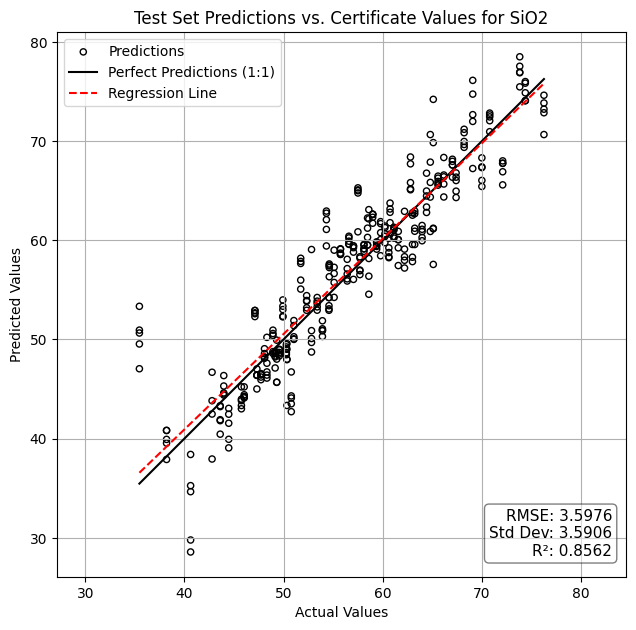
\includegraphics[width=\textwidth]{images/one_to_one/enetalpha01/SiO2.png}
            \end{subfigure} & \hspace{3cm}
            \begin{subfigure}{0.5\textwidth}
                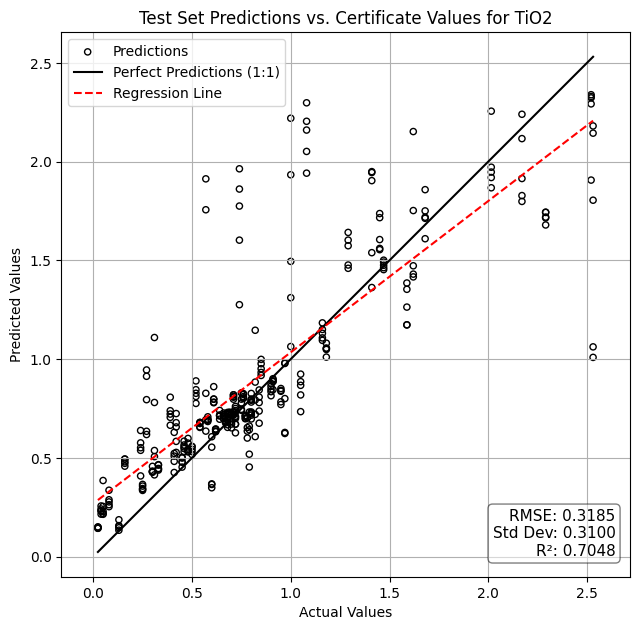
\includegraphics[width=\textwidth]{images/one_to_one/enetalpha01/TiO2.png}
            \end{subfigure} \\
            \begin{subfigure}{0.5\textwidth}
                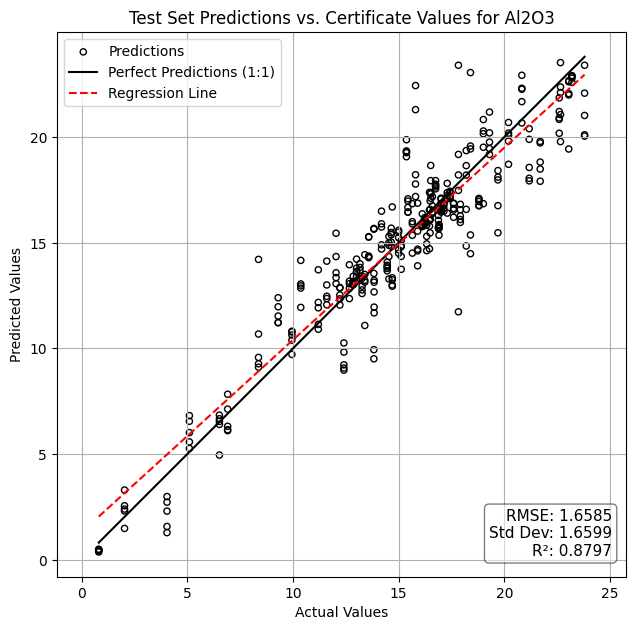
\includegraphics[width=\textwidth]{images/one_to_one/enetalpha01/Al2O3.png}
            \end{subfigure} & \hspace{3cm}
            \begin{subfigure}{0.5\textwidth}
                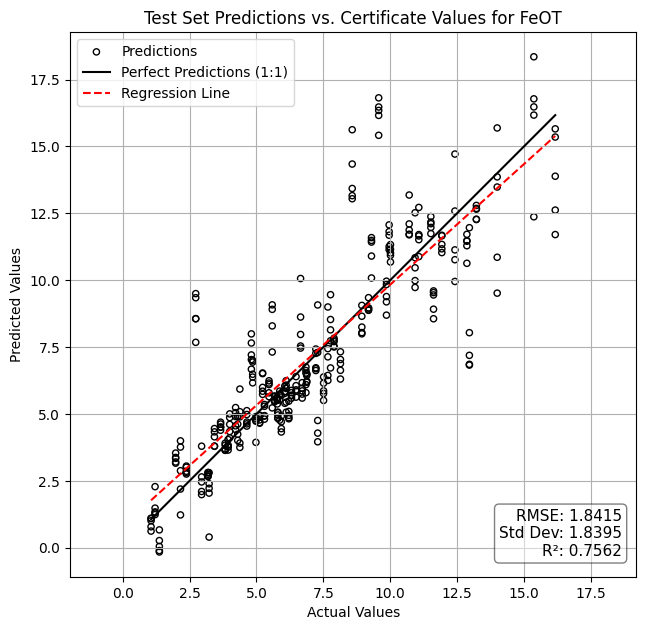
\includegraphics[width=\textwidth]{images/one_to_one/enetalpha01/FeOT.png}
            \end{subfigure} \\
            \begin{subfigure}{0.5\textwidth}
                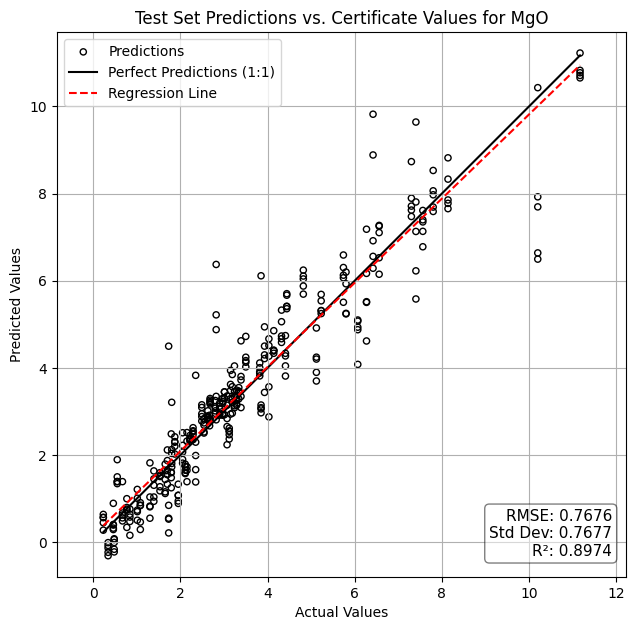
\includegraphics[width=\textwidth]{images/one_to_one/enetalpha01/MgO.png}
            \end{subfigure} & \hspace{3cm}
            \begin{subfigure}{0.5\textwidth}
                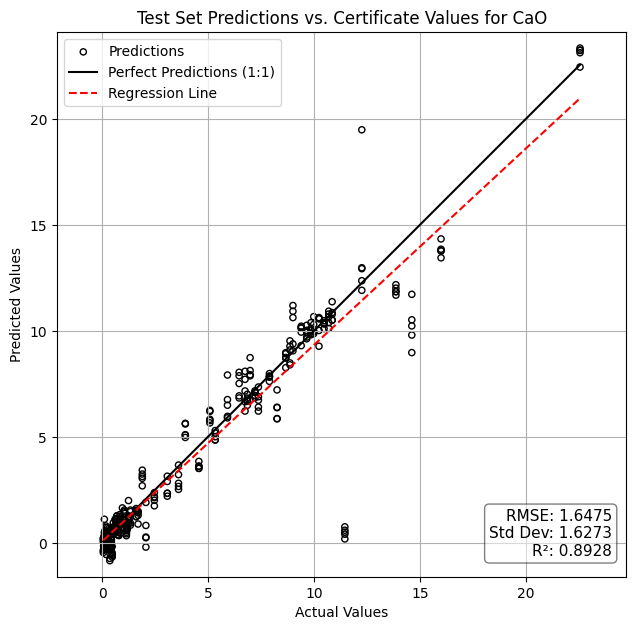
\includegraphics[width=\textwidth]{images/one_to_one/enetalpha01/CaO.png}
            \end{subfigure} \\
            \begin{subfigure}{0.5\textwidth}
                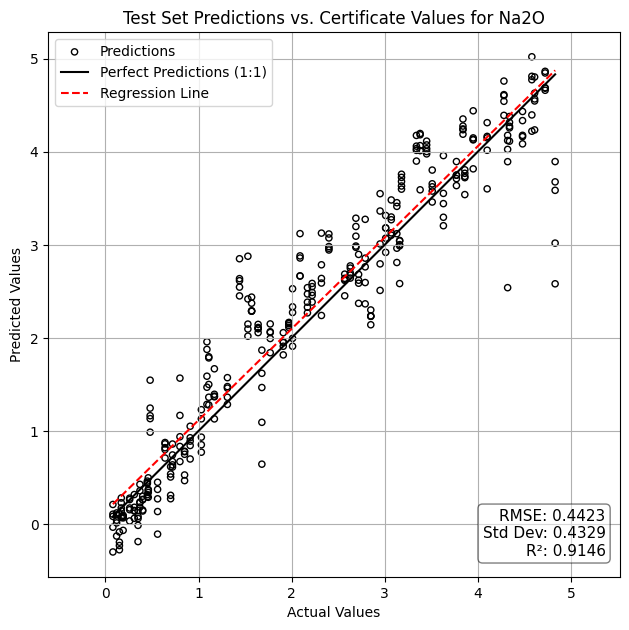
\includegraphics[width=\textwidth]{images/one_to_one/enetalpha01/Na2O.png}
            \end{subfigure} & \hspace{3cm}
            \begin{subfigure}{0.5\textwidth}
                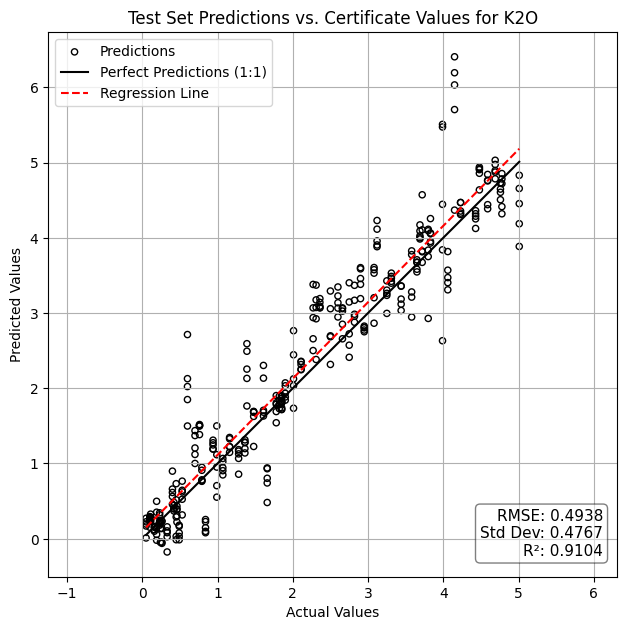
\includegraphics[width=\textwidth]{images/one_to_one/enetalpha01/K2O.png}
            \end{subfigure}
        \end{tabular}
    }
    \caption{One-to-one plots for the stacking ensemble model with the \gls{enet} as the meta-learner with $\alpha = 0.1$.}
    \label{fig:enetalpha01_one_to_one}
\end{figure*}

\begin{figure*}
    \centering
    \resizebox{0.75\textwidth}{!}{
        \begin{tabular}{cc}
            \begin{subfigure}{0.5\textwidth}
                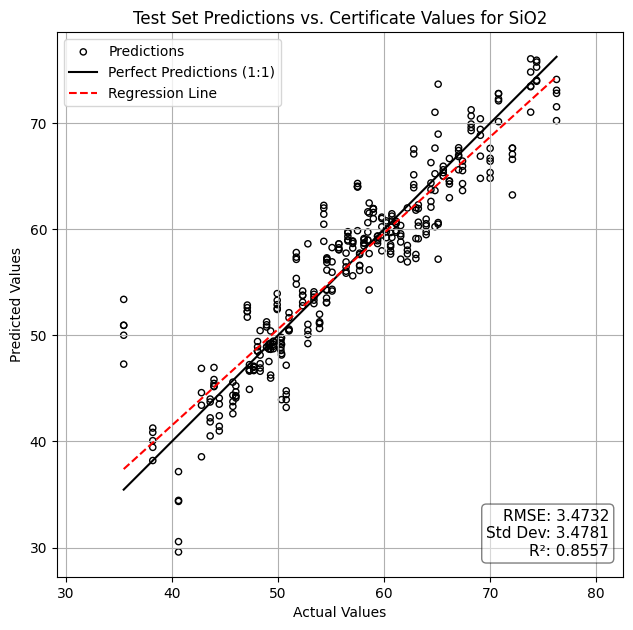
\includegraphics[width=\textwidth]{images/one_to_one/svr/SiO2.png}
            \end{subfigure} & \hspace{3cm}
            \begin{subfigure}{0.5\textwidth}
                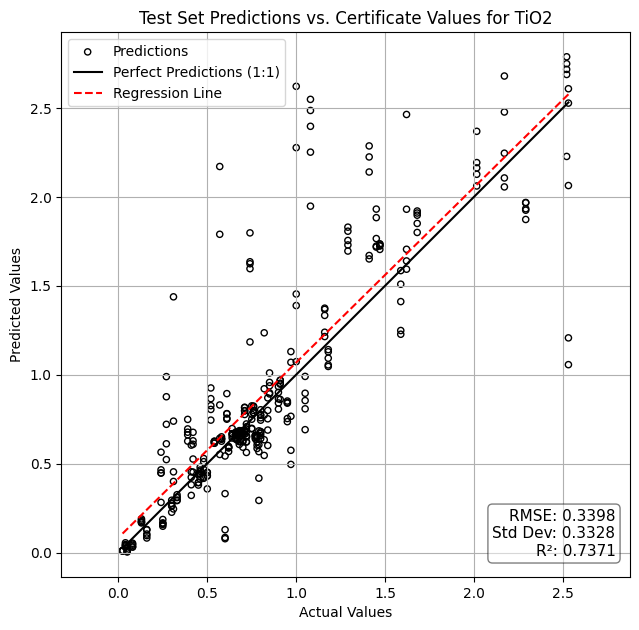
\includegraphics[width=\textwidth]{images/one_to_one/svr/TiO2.png}
            \end{subfigure} \\
            \begin{subfigure}{0.5\textwidth}
                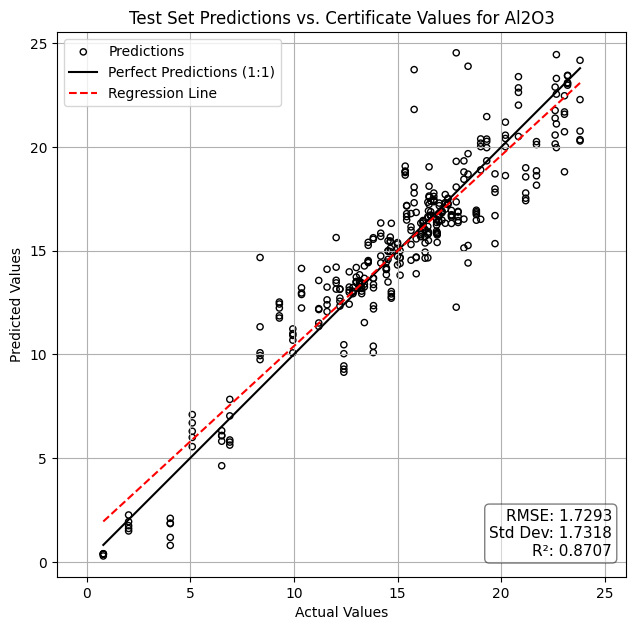
\includegraphics[width=\textwidth]{images/one_to_one/svr/Al2O3.png}
            \end{subfigure} & \hspace{3cm}
            \begin{subfigure}{0.5\textwidth}
                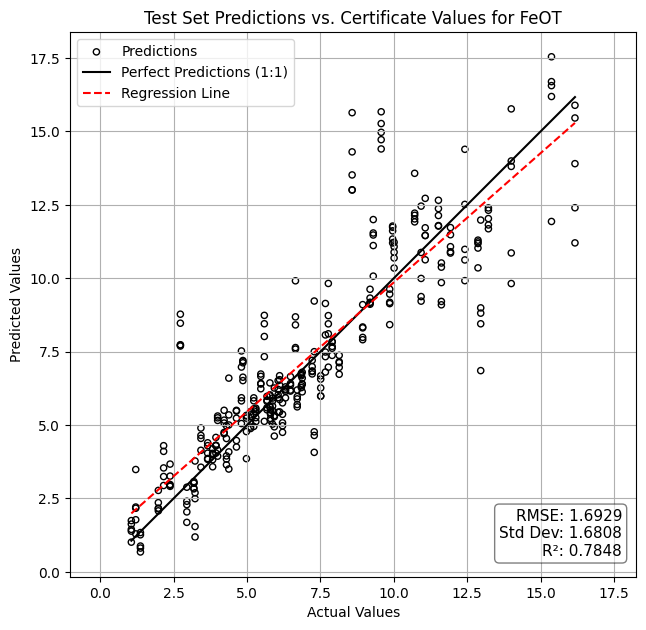
\includegraphics[width=\textwidth]{images/one_to_one/svr/FeOT.png}
            \end{subfigure} \\
            \begin{subfigure}{0.5\textwidth}
                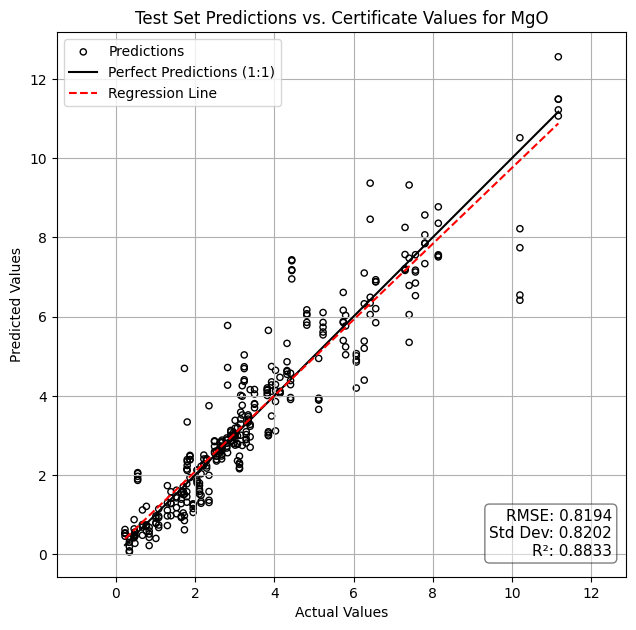
\includegraphics[width=\textwidth]{images/one_to_one/svr/MgO.png}
            \end{subfigure} & \hspace{3cm}
            \begin{subfigure}{0.5\textwidth}
                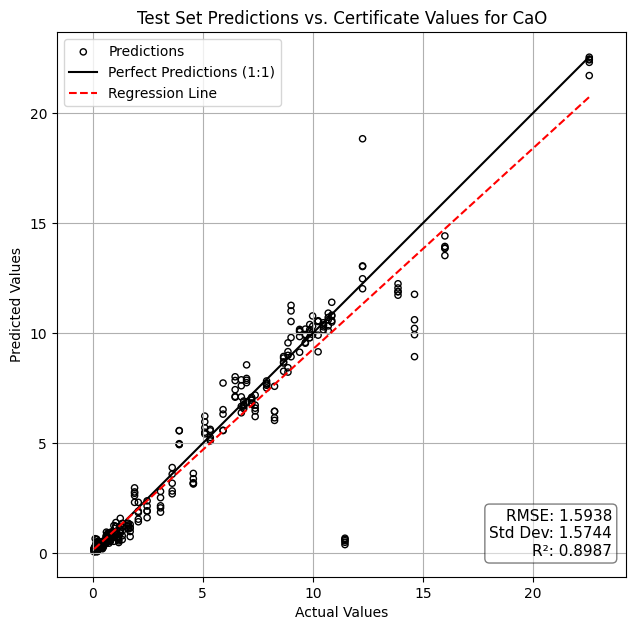
\includegraphics[width=\textwidth]{images/one_to_one/svr/CaO.png}
            \end{subfigure} \\
            \begin{subfigure}{0.5\textwidth}
                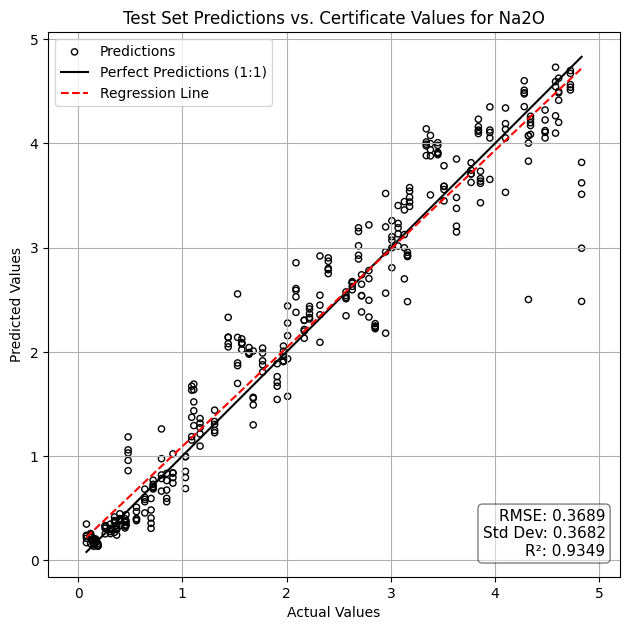
\includegraphics[width=\textwidth]{images/one_to_one/svr/Na2O.png}
            \end{subfigure} & \hspace{3cm}
            \begin{subfigure}{0.5\textwidth}
                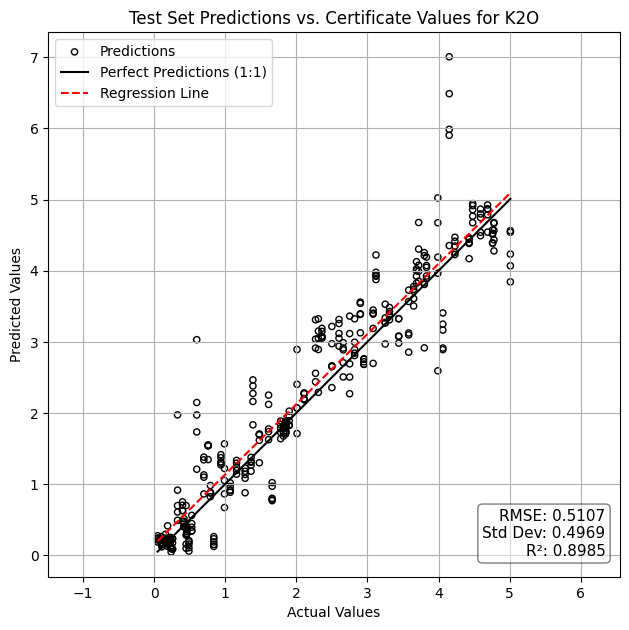
\includegraphics[width=\textwidth]{images/one_to_one/svr/K2O.png}
            \end{subfigure}
        \end{tabular}
    }
    \caption{One-to-one plots for the stacking ensemble model with the \gls{svr} as the meta-learner}
    \label{fig:svr_one_to_one}
\end{figure*}
